\documentclass[conference]{IEEEtran}

\usepackage{pythonhighlight}

\usepackage{graphicx}
\usepackage{hyperref}
\usepackage{float}
\usepackage[english]{babel}
\usepackage{listings} % code blocks
\usepackage[utf8]{inputenc}
\usepackage{amsmath}
\usepackage[acronym]{glossaries}
\makeglossaries
%\usepackage{etoolbox} % citações

\hyphenation{}

\begin{document}
% paper title
% can use linebreaks \\ within to get better formatting as desired
\title{Heart Disease Detection Using Machine Learning}

% author names and affiliations
% use a multiple column layout for up to three different
% affiliations
\author{
    \IEEEauthorblockN{Nelson Loureiro}
   \IEEEauthorblockA{
        Fundamentos de Aprendizagem Automática 24/25\\
        Departamento de Eletrónica, Telecomunicações e Informática\\
        University of Aveiro\\
        Aveiro, Portugal\\
        nelson.loureiro@ua.pt
    }
    \and
    \IEEEauthorblockN{Cristiano Nicolau}
    \IEEEauthorblockA{
        Fundamentos de Aprendizagem Automática 24/25\\
        Departamento de Eletrónica, Telecomunicações e Informática\\
        University of Aveiro\\
        Aveiro, Portugal\\
        cristianonicolau@ua.pt
    }
}
% make the title area
\maketitle

\begin{abstract}
The main goal of this project is to apply machine learning algorithms, as learned in class, to solve a specific data science problem: developing models capable of predicting whether a patient has heart disease or not. Using a variety of machine learning techniques, the project aims to optimize model accuracy in classifying patients into "diseased" or "healthy" categories based on clinical data. In this report, we focus on fine-tuning the models to achieve the best performance, evaluating their effectiveness using various classification metrics and ensuring robust predictions to assist in early detection and diagnosis of heart disease.
\end{abstract}

\begin{center}
    \textit{\textbf{Keywords} — Machine Learning, Classification Model, Logistic Regression, SVM, Neural Network, Normalization}
\end{center}
\IEEEpeerreviewmaketitle
%\acrlong{da}
%\acrshort{da}
%\acrfull{da}

\newacronym{ml}{ML}{Machine Learning}
\newacronym{svm}{SVM}{Support Vector Machine} 
\newacronym{mlp}{MLP}{Multi-layer Perceptrons}
\newacronym{fnn}{FNN}{Feedforward Neural Network}
\newacronym{TP}{TP}{True Positive}
\newacronym{FP}{FP}{False Positive}
\newacronym{TN}{TN}{True Negative}
\newacronym{FN}{FN}{False Negative}

\section{Introduction}
\label{sec:Introduction}
Heart disease remains one of the most significant causes of mortality worldwide, affecting millions of people each year. Early detection and treatment are essential in preventing severe complications, improving life expectancy, and enhancing the quality of life for those at risk. By leveraging data-driven techniques and machine learning algorithms, we can support healthcare professionals by predicting the likelihood of heart disease in patients based on clinical and demographic characteristics, facilitating quicker and more accurate diagnoses.

This project focuses on the Cleveland Heart Disease Dataset, a widely recognized benchmark in medical and machine learning research. This dataset, sourced from the UCI Machine Learning Repository, includes clinical data collected from multiple databases (Cleveland, Hungary, Switzerland, and Long Beach V). However, only the Cleveland subset will be used in this analysis, as it is the most commonly utilized in published studies and provides a reliable basis for heart disease prediction.

The Cleveland subset comprises fourteen selected attributes that reflect relevant demographic and clinical variables, such as age, cholesterol levels, blood pressure, and other factors often associated with heart disease. The target variable, `target`, indicates the presence (1) or absence (0) of heart disease. Our objective is to apply machine learning algorithms to classify patients as either "diseased" or "healthy" based on these attributes. By identifying high-risk individuals more effectively, this project aims to enhance diagnostic processes and enable more targeted treatment strategies.

\section{State of the Art} \label{sec}
\acrfull{ml} has become a fundamental tool in healthcare, especially in disease prediction and diagnosis. By analyzing large volumes of clinical data, \acrshort{ml} models can identify complex patterns that can aid in predicting medical conditions and support decision-making by healthcare professionals. However, the application of \acrshort{ml} in healthcare presents specific challenges, particularly related to model accuracy, interpretability, and reliability. This state of the art section provides an overview of the use of \acrshort{ml} in healthcare, its limitations and challenges, its specific application in the diagnosis of heart diseases, and some of the training approaches and techniques that will be used in this work.

\subsection{Machine Learning in Health Predictions}
In healthcare, machine learning is widely used to create predictive models that assist in the diagnosis and prognosis of diseases, particularly chronic conditions such as diabetes, cancer, and cardiovascular diseases. Predictive models in healthcare need to handle complex data, which may include clinical, demographic, and lifestyle variables of patients. Studies have shown that the use of \acrshort{ml} can improve diagnostic accuracy, but it is essential that these models are interpretable, allowing doctors and specialists to understand the determining factors behind each prediction. However, a recurring problem is class imbalance, where less common diseases are underrepresented in the data, causing the model to be biased toward the dominant class (e.g., healthy patients). In our project, these aspects will be considered when applying \acrshort{ml} for predicting heart diseases.

\subsection{Application of \acrshort{ml} in Heart Disease Prediction}
In the specific context of heart disease prediction, the use of machine learning appears promising in helping identify high-risk patients, enabling preventive interventions. Several studies have already applied \acrshort{ml} algorithms, such as logistic regression, decision trees, and neural networks, to classify the presence of heart disease from clinical data. In our work, we will focus on the \textit{Cleveland Heart Disease Dataset}, a widely used dataset in medical research and ML studies to study and predict the presence of heart disease. This dataset includes variables such as age, blood pressure, cholesterol, and other clinical factors associated with heart risk. Using algorithms such as \textit{Support Vector Classifier (SVC)}, \textit{Logistic Regression}, and \textit{Multi-Layer Perceptron (MLP)}, the goal is to build models that can classify patients as “diseased” or “healthy” with high accuracy.

\subsection{Model Training and Validation Techniques}
To ensure the reliability of the models, it is essential to split the data into training, validation, and test sets. In this project, we will apply the \textit{k-fold cross-validation} technique, which divides the data into multiple training and testing subsets, promoting a more robust evaluation. This method helps prevent overfitting, ensuring that the model generalizes well to new data. During training, the model’s cost function will be monitored throughout the iterations, with graphical visualizations to check the trajectory and convergence of the cost function, both with and without regularization, to better understand the models' behavior.

\subsection{Systematic Hyperparameter Selection}
Choosing the right hyperparameters is a crucial step in developing effective predictive models. Instead of relying on randomly chosen values, this project will adopt a systematic approach to hyperparameter selection, using techniques like \textit{GridSearchCV} and \textit{RandomizedSearchCV}. \textit{GridSearchCV} performs an exhaustive search by testing predefined combinations of hyperparameters in a grid and selecting the best values based on maximizing the model’s accuracy. This approach allows for a comprehensive exploration of different hyperparameter configurations, such as regularization strength and the number of neurons in the MLP’s hidden layer.

On the other hand, \textit{RandomizedSearchCV} offers a more efficient alternative when the search space is very large. Instead of testing all possible combinations, \textit{RandomizedSearchCV} randomly selects a fixed number of hyperparameter combinations from specified distributions, which can significantly reduce computation time while maintaining the chance of finding effective combinations.

These two approaches will be applied to the three selected models (\textit{SVC}, \textit{Logistic Regression}, and \textit{MLP}), aiming to optimize their performance. Combining these hyperparameter selection techniques will provide a robust and efficient evaluation of the models, allowing each algorithm to be tuned to achieve the best possible performance.

\subsection{Model Evaluation: Confusion Matrix and Classification Metrics}
The evaluation of the models will be carried out using the confusion matrix, which provides a detailed view of the model’s correct and incorrect predictions for each class (patients with and without disease). In addition, classification metrics including \textit{accuracy}, \textit{precision}, \textit{recall}, and \textit{F1-score} will be calculated. These metrics are essential for assessing the effectiveness of the model. 

\subsubsection{Recall (Sensitivity)}
Recall is perhaps the most important metric in solving the classification task of this project, that is because it measures the proportion of actual cancer cases that the model correctly identifies. It answers the question: "Out of all patients who truly have cancer, how many did the model detect?". Its formula is the following:
\[Recall=\frac{True Positives (TP)}{True Positives (TP)+False Negatives (FN)}\]
Missing a cancer diagnosis (false negative) can have severe consequences, as early detection is often crucial for effective treatment. A model with low recall might overlook cases of cancer, leading to delayed or missed treatments.
In contrast, a false positive (predicting cancer when it's not present) can cause stress and lead to additional tests, but it is generally less harmful than a false negative.

\subsubsection{Precision}
The precision score is a performance metric used to evaluate the accuracy of a classification model, particularly in binary and multi-class classification problems. It measures the proportion of correctly predicted positive observations to the total predicted positive observations. Precision answers the question: "Of all the instances that were predicted as positive, how many were actually positive?" Its formula is:
\[Precision=\frac{True Positives (TP)}{True Positives (TP)+False Positives (FP)}\]

\subsubsection{F1-Score}
The F1-score, being the harmonic mean (represented below) between precision and recall, will be one of the most important metrics, as it provides a balance between the model’s ability to correctly identify diseased patients and avoid false positives, ensuring that the model is effective both in detecting disease and minimizing diagnostic errors.
\[F1Score=2 \times \frac{Precision*Recall}{Precision+Recall}\]

\subsubsection{Accuracy}
Accuracy is the proportion of correct predictions (both true positives and true negatives) to the total number of predictions made. It represents the overall correctness of the model's predictions. It is especially usefull when the dataset is balanced.

\subsection{Current Challenges and Future Perspectives}
Despite the advancements, the use of machine learning for predicting heart disease faces several challenges. One of the main issues is class imbalance, where the majority of patients in the data belong to the healthy class, which can lead to biased models. Additionally, the interpretability of more complex models, such as neural networks, remains a limitation, as healthcare professionals need to understand the reasoning behind the predictions. One technique that could be used is the application of \textit{deep learning} methods to capture more complex patterns, along with the integration of real-time data, which could enhance model accuracy and enable even more dynamic diagnoses.
\section{Machine Learning Models}
\label{sec:ML_Models}
\subsection{Introduction}
This section describes all of the \acrfull{ml} algorithms that were implemented in the project. These models are in the supervised group of \acrshort{ml} algorithms.

\subsection{Logistic Regression}
Despite its name, Logistic Regression is not a regression but rather a classification algorithm.
It predicts the probability that an instance belongs to a particular class. For binary classification, the output is typically a probability value between 0 and 1, which can be converted into class labels (e.g., 0 or 1, 'cancer' or 'not cancer') using a threshold (usually 0.5).

The logistic regression maps any input to a value between 0 and 1 by applying the sigmoid function as seen in figure \ref{fig:logistic_reg}. In this figure \(h_\theta\) is the output of the \(\theta\) parameters matrix and x the matrix of the inputs.
\begin{figure}[!htb]
    \centering
    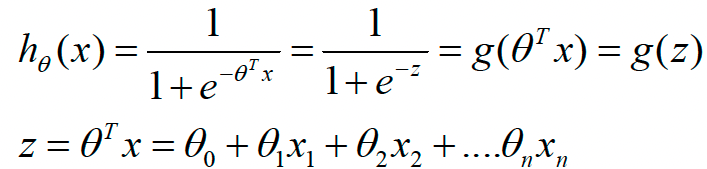
\includegraphics[width=0.8\linewidth]{images/logistic_reg.png}
    \caption{Logistic Regression model definition.}
    \label{fig:logistic_reg}
\end{figure}

Usually the threshold defined for this model is 0.5 and based on it, the probability is converted into a discrete class (e.g., if the probability is higher than 0.5 than class 'cancer', if it's lower class 'not cancer'). The Logistic Regression aims at minimizing its loss function which is the 'Binary Cross-Entropy' or Log Loss function. This function measures the difference between the predicted probability of each data point and its true label, and is represented at figure \ref{fig:loss_log_reg}.
\begin{figure}[!htb]
    \centering
    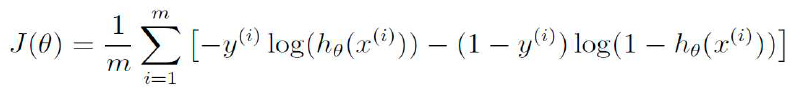
\includegraphics[width=0.9\linewidth]{images/loss_log_reg.png}
    \caption{Binary Cross-Entropy loss function.}
    \label{fig:loss_log_reg}
\end{figure}

The Logistic Regression works well with linearly separable data. When it is not the case, it can still be the solution if combined with feature engineering. Overall, it is a model which is easy to interpret, simple, and effective.

\subsection{Support Vector Machine (SVM)}
The \acrfull{svm} is a model that can be used for solving both classification and regression tasks, even though it is most used in classification. For classification this model takes into consideration the closest data points from each class, and determines a hyperplane that maximally separates classes while ensuring the margin (distance between the hyperplane and the nearest data points from each class) is as large as possible as illustrated in image \ref{fig:svm_supp_vectors}.
\begin{figure}[!htb]
    \centering
    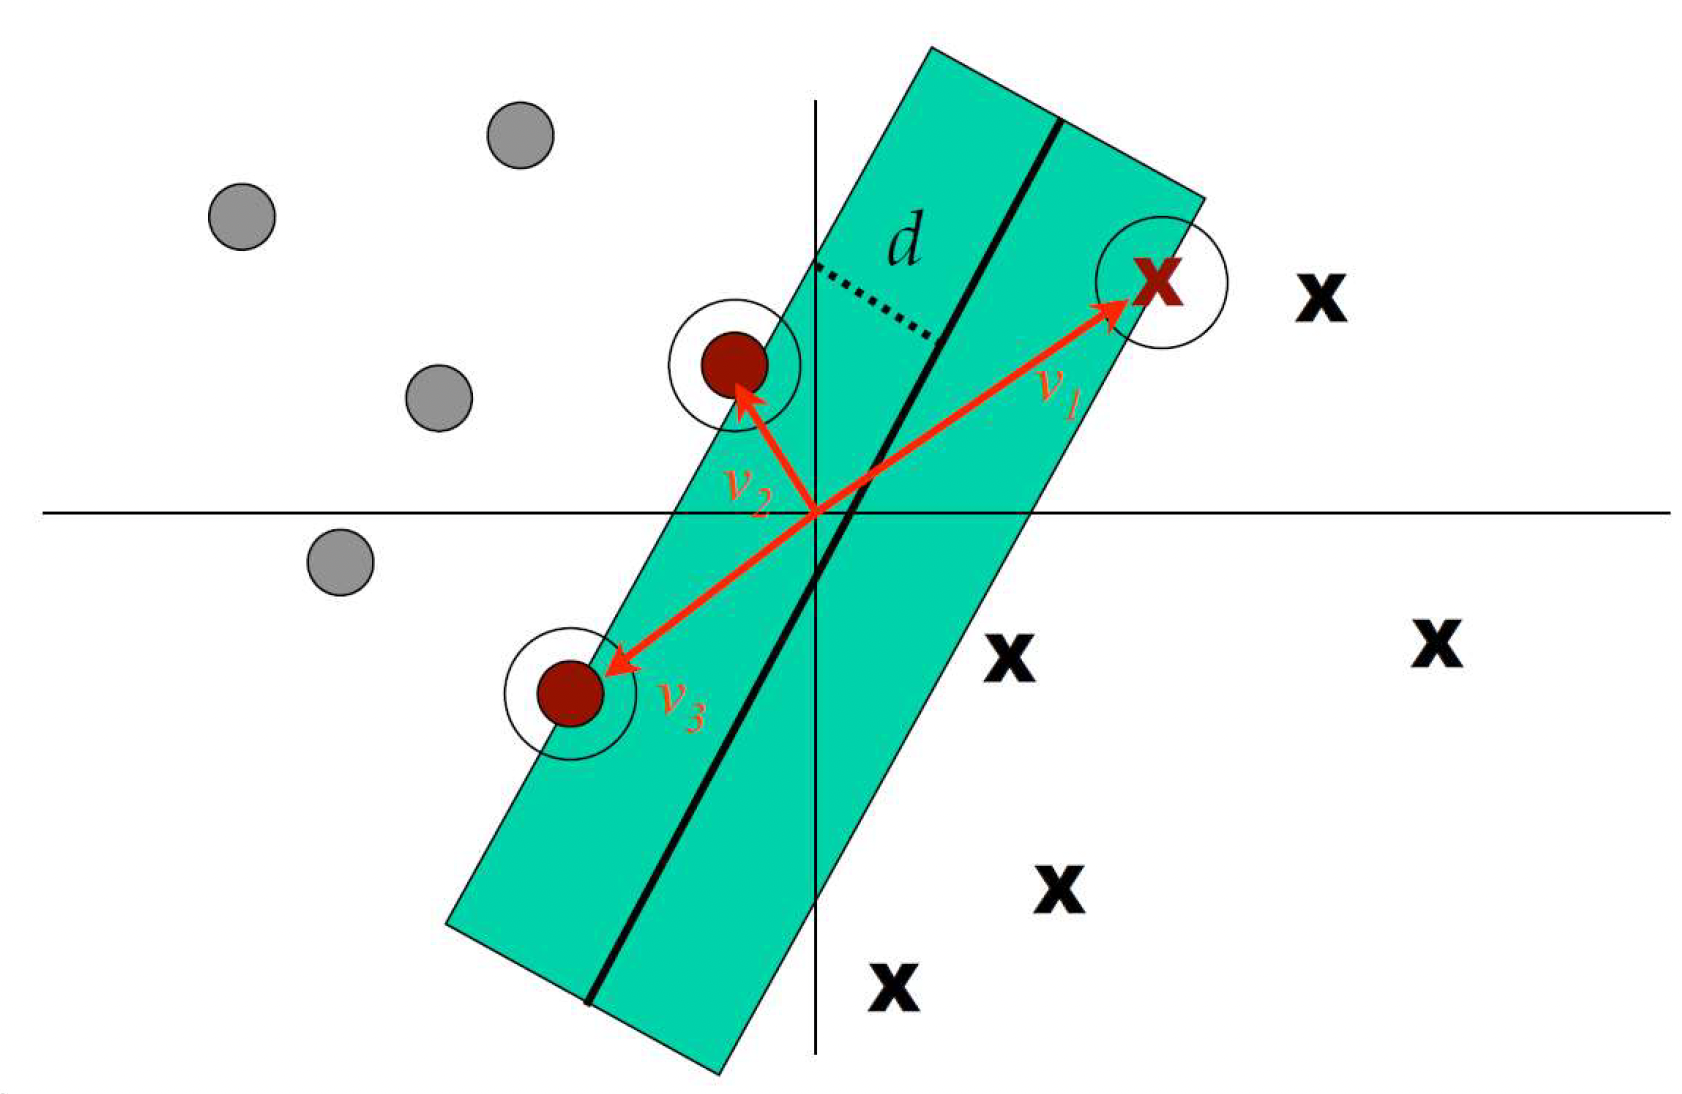
\includegraphics[width=0.9\linewidth]{images/svm.png}
    \caption{Support vectors of \acrshort{svm}.}
    \label{fig:svm_supp_vectors}
\end{figure}

Each closest point of each class represents a \textbf{support vector} which determines the position and orientation of the hyperplane, making \acrshort{svm} highly robust to the influence of other data points.
\acrshort{svm} tries to minimise two errors: \begin{itemize}
    \item Classification error: how many points are wrongly classified
    \item Margin error: optimise the margin among classes
\end{itemize}
This algorithm searches for the largest margin that minimises the classification error. Regarding the classification error the \acrshort{svm} uses a modification of LogReg cost function with two assimptotic safety margins that are computationally more advantageous.

When data is not linearly separable, a kernel trick is applied on it. A kernel is a function that maps a lower-dimensional data into higher dimensional data.

\subsection{Multi-layer Perceptrons (MLP)}
A \acrfull{mlp} is a type of \acrfull{fnn} that is widely used in supervised learning tasks, including classification and regression.
The architecture of a \acrshort{mlp} model consists of an input layer composed by nodes where each node represents a feature of the input data; one or more hidden layers where each neuron receives inputs from all neurons in the previous layer (either the input layer or another hidden layer) and produces an output that is passed to the next layer. Hidden layers are layers between the input and output layers. The architecture of this model ends with an output layer on which the number of neurons depend on the task at hand. In binary classification, there may be two neurons representing the probability of belonging to one class; while in multi-class classification tasks, there can be multiple neurons in the output layer.

Each neuron computes a weighted sum of its inputs, adds a bias term, and applies an activation function (e.g., ReLU, sigmoid) to introduce nonlinearity. This enables the network to model complex relationships. During training, the model learns optimal weights and biases by minimizing a loss function (e.g., cross-entropy for classification) through a process called backpropagation. Backpropagation calculates the gradients of the loss with respect to the weights, which are then updated using optimization algorithms like Stochastic Gradient Descent (SGD) or Adam to iteratively improve performance.
\section{Data Visualization}
\label{sec:Data Visualization}
\subsection{Dataset Description}
The Cleveland Heart Disease Dataset\cite{HeartDiseaseCleveland} originally contains 76 attributes; however, we use a preprocessed standard subset\cite{HeartDiseaseKaggle} of 13 attributes, widely utilized in published experiments with this dataset. This subset includes relevant demographic and clinical variables, described below:

The variable Age refers to the patient’s age in years, while Sex indicates the gender (1 for male, 0 for female). The type of chest pain experienced is categorized by the variable CP (Chest Pain Type), which has four categories: typical angina, atypical angina, non-anginal pain, and asymptomatic. Resting blood pressure, measured in mm Hg, is represented by Trestbps (Resting Blood Pressure), while Chol (Serum Cholesterol) records serum cholesterol levels in mg/dl.

Fasting blood sugar levels greater than 120 mg/dl are indicated by FBS (Fasting Blood Sugar), where 1 denotes true and 0 false. Resting electrocardiographic results are described by the variable Restecg (Resting Electrocardiographic Results), with values of 0 for normal, 1 for ST-T wave abnormalities, and 2 for left ventricular hypertrophy. The maximum heart rate achieved is recorded in the variable Thalach (Maximum Heart Rate Achieved), and the presence of exercise-induced angina is indicated by Exang (Exercise-Induced Angina) (1 for yes, 0 for no).

The variable Oldpeak measures ST-segment depression induced by exercise relative to rest, and Slope indicates the slope of the peak exercise ST segment. The number of major vessels (0–3) colored by fluoroscopy is indicated by the variable Ca (Number of Major Vessels Colored by Fluoroscopy), and the thalassemia test result is represented by Thal (Thalassemia Test Result), with values 3 for normal, 6 for a fixed defect, and 7 for a reversible defect. Finally, the Target variable is the outcome, indicating the presence (1) or absence (0) of heart disease.

The final column, denoted as "Target," serves as the pivotal indicator of the presence of heart disease, where a value of "0" signifies the absence of heart disease and "1" indicates its presence.

The Figure 4, illustrates the distribution of the features in the dataset, allowing us to understand their variability and potential influence on the classification task.

\begin{figure}[H]
    \centering
    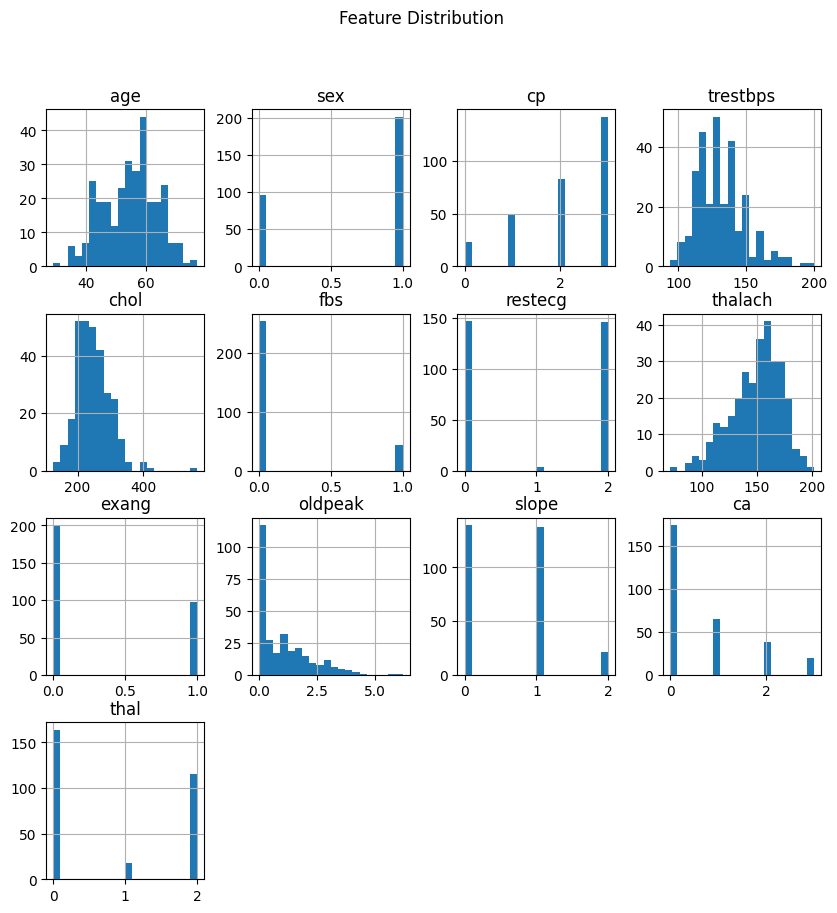
\includegraphics[width=1\linewidth]{images/feature_destribution.png}
    \caption{Feature Distribution}
    \label{fig:enter-label}
\end{figure}

\subsection{Dataset Balancing}

To gain a deeper understanding of the dataset, it is crucial to utilize various data visualization techniques, such as box plots, histograms, and scatter plots. These visualizations offer valuable insights into the relationships between variables and help identify potential patterns or correlations within the data.

The first visualization, shown in Fig. 5, is a histogram that illustrates the distribution of heart disease cases in the dataset. This histogram reveals a nearly balanced distribution, with a slight majority of patients not having heart disease. As seen in the figure, there are 160 patients without heart disease and 137 patients with heart disease, making the target variable relatively balanced. A balanced dataset is crucial for model training, as it reduces the risk of bias toward the majority class and increases the likelihood of accurate predictions.

\begin{figure}[ht] \centering 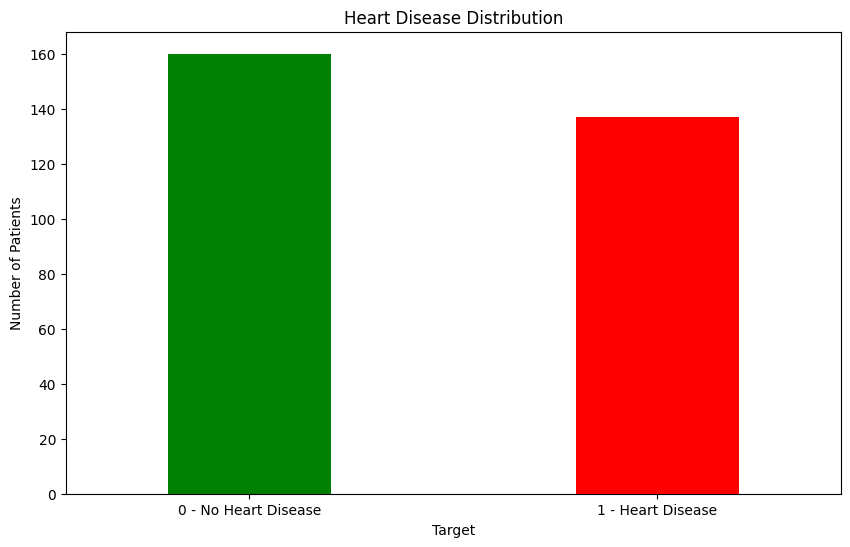
\includegraphics[width=0.8\linewidth]{images/hist_heart_desease_distribution.png} \caption{Histogram of Heart Disease Distribution} \label{fig:heart_disease_histogram} \end{figure}

The next visualization, Fig. 6, displays the distribution of patients with and without heart disease in a circular format (pie chart). This provides a clearer view of the proportions of each class. The dataset is balanced, with 53.87\% of patients without heart disease and 46.13\% of patients with heart disease.

\begin{figure}[ht] \centering 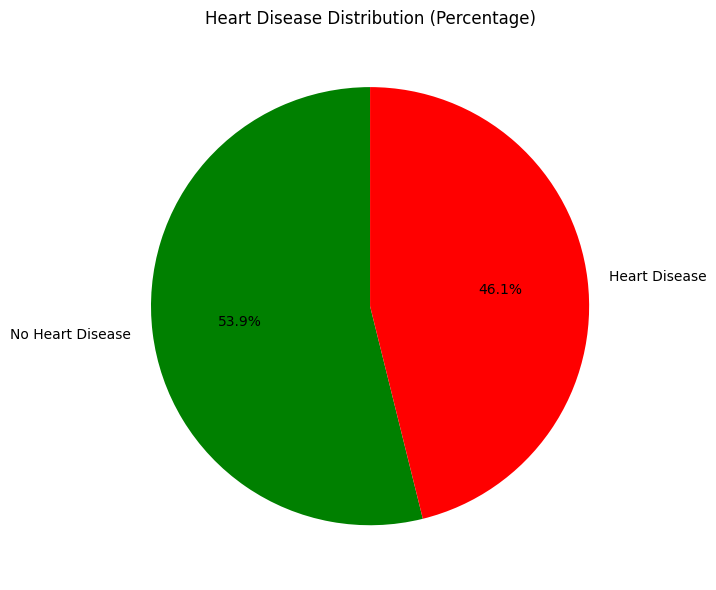
\includegraphics[width=0.75\linewidth]{images/heart_distribution_circular.png} \caption{Heart Disease Distribution (Percentage)} \label{fig:heart_disease_pie_chart} \end{figure}

This balance is important to ensure that the model does not develop a bias towards predicting the majority class, allowing for more accurate and fair predictions.

\subsection{Comparison of Age and Sex Distribution in the Dataset}
The age distribution, Fig. 7, shows that the average age of the patients is 54.54 years, with the median being 56 years, and the most frequent age (mode) being 58 years. The age range spans from 29 years to 77 years, indicating a relatively broad age distribution within the dataset. This diversity in age is important for creating a model that can effectively predict heart disease across different age groups.

\begin{figure}[ht]
    \centering
    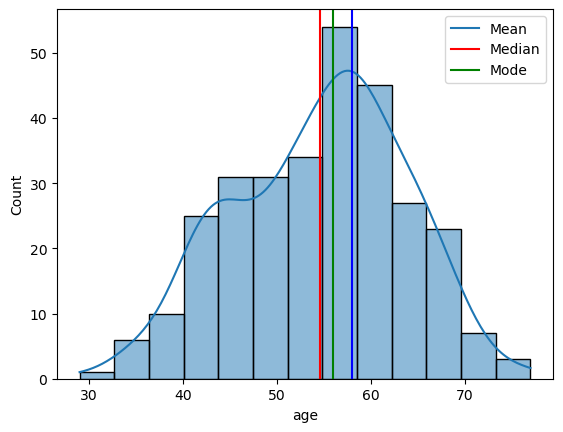
\includegraphics[width=0.8\linewidth]{images/age_distribution.png}
    \caption{Age Distribution}
    \label{fig:enter-label}
\end{figure}
\hfill \break

Notably, a significant number of patients fall within the 40 to 70-year-old range, which is typically the period when heart diseases are more commonly diagnosed. This trend is consistent with general medical knowledge, as the risk of heart disease increases with age, particularly after the age of 40. Contributing factors include the accumulation of cardiovascular risk factors over the years, such as high blood pressure, cholesterol levels, and lifestyle choices. This concentration of patients in the 40–70 age range suggests that the dataset captures a critical age group for heart disease prediction.

\begin{figure}[ht]
    \centering
    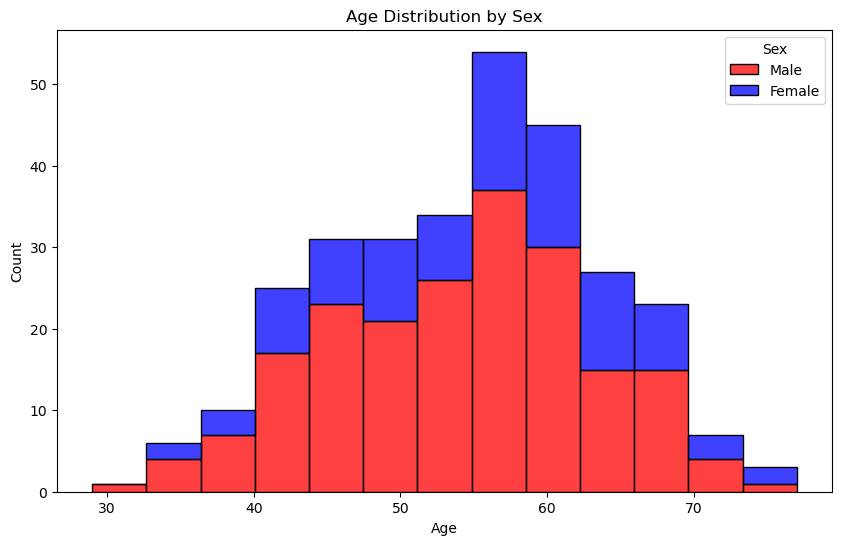
\includegraphics[width=0.8\linewidth]{images/women_men.png}
    \caption{Age distribution by Sex}
    \label{fig:enter-label}
\end{figure}

When we look at the age distribution by sex on figure 8, we observe that the dataset contains 201 men (67.7\% of the total) and 96 women (32.3\% of the total). This reveals a higher representation of men in the dataset. Men, on average, are more likely to develop heart disease than women, which is reflected in the dataset's demographic distribution.

\begin{figure}[ht]
    \centering
    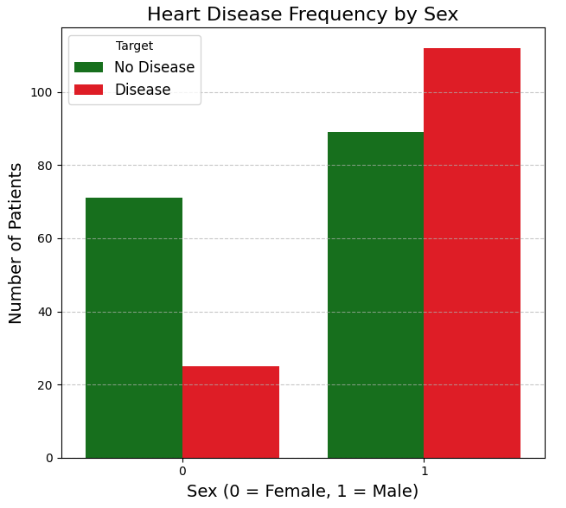
\includegraphics[width=0.75\linewidth]{images/freq_heart_disease_by_sex.png}
    \caption{Heart Disease Distribution by Sex }
    \label{fig:enter-label}
\end{figure}

Among the men, 55.7\% have heart disease, while 44.3\% do not. In contrast, among the women, only 26.0\% have heart disease, with the remaining 74.0\% without it. These figures highlight that heart disease is more prevalent among men in this dataset, which is consistent with general clinical findings that heart disease tends to affect men at a higher rate.
%\hfill \break
\begin{figure}[H]
    \centering
    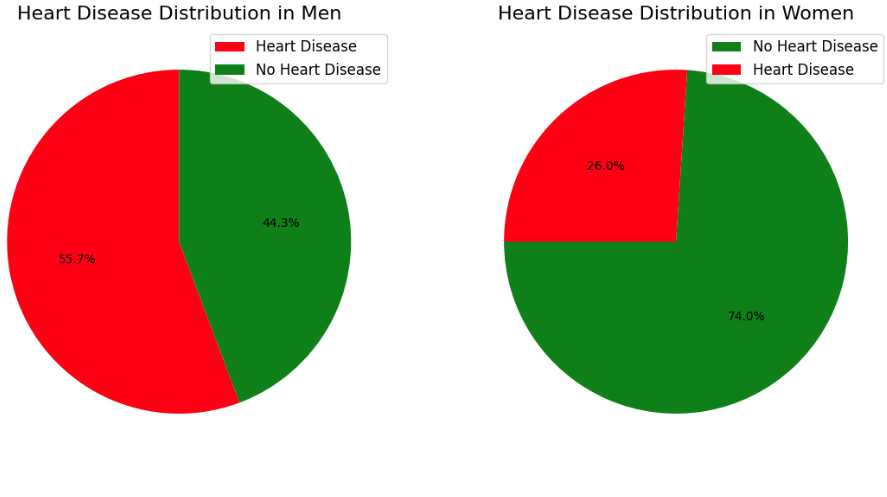
\includegraphics[width=1\linewidth]{images/perc_disease_by_sex.png}
    \caption{Heart Disease Distribution by Sex (Percentage)}
    \label{fig:enter-label}
\end{figure}

Further examining the age distribution within each sex, we can observe how age interacts with heart disease for both men and women. Heart disease is present in a notable portion of the male and female population particularly in the older age groups. While heart disease is less common in women overall, it is still present in a notable portion of the female population.

In summary, the data shows that men are more likely to have heart disease than women, and age plays an important role in the development of the disease for both genders. This insight helps us understand the potential impact of age and sex on heart disease prediction models and may guide future analyses on how to best predict heart disease based on these factors.

\subsection{Attribute Distributions and Their Relationship with Heart Disease} 

The dataset reveals notable differences in the distributions of key attributes between patients with and without heart disease, as seen in figure 11 and 12. These distinctions highlight critical factors that may be associated with the presence of heart disease, providing valuable insights for diagnosis, risk assessment, and preventive strategies.

\begin{figure}[!htb]
    \centering
    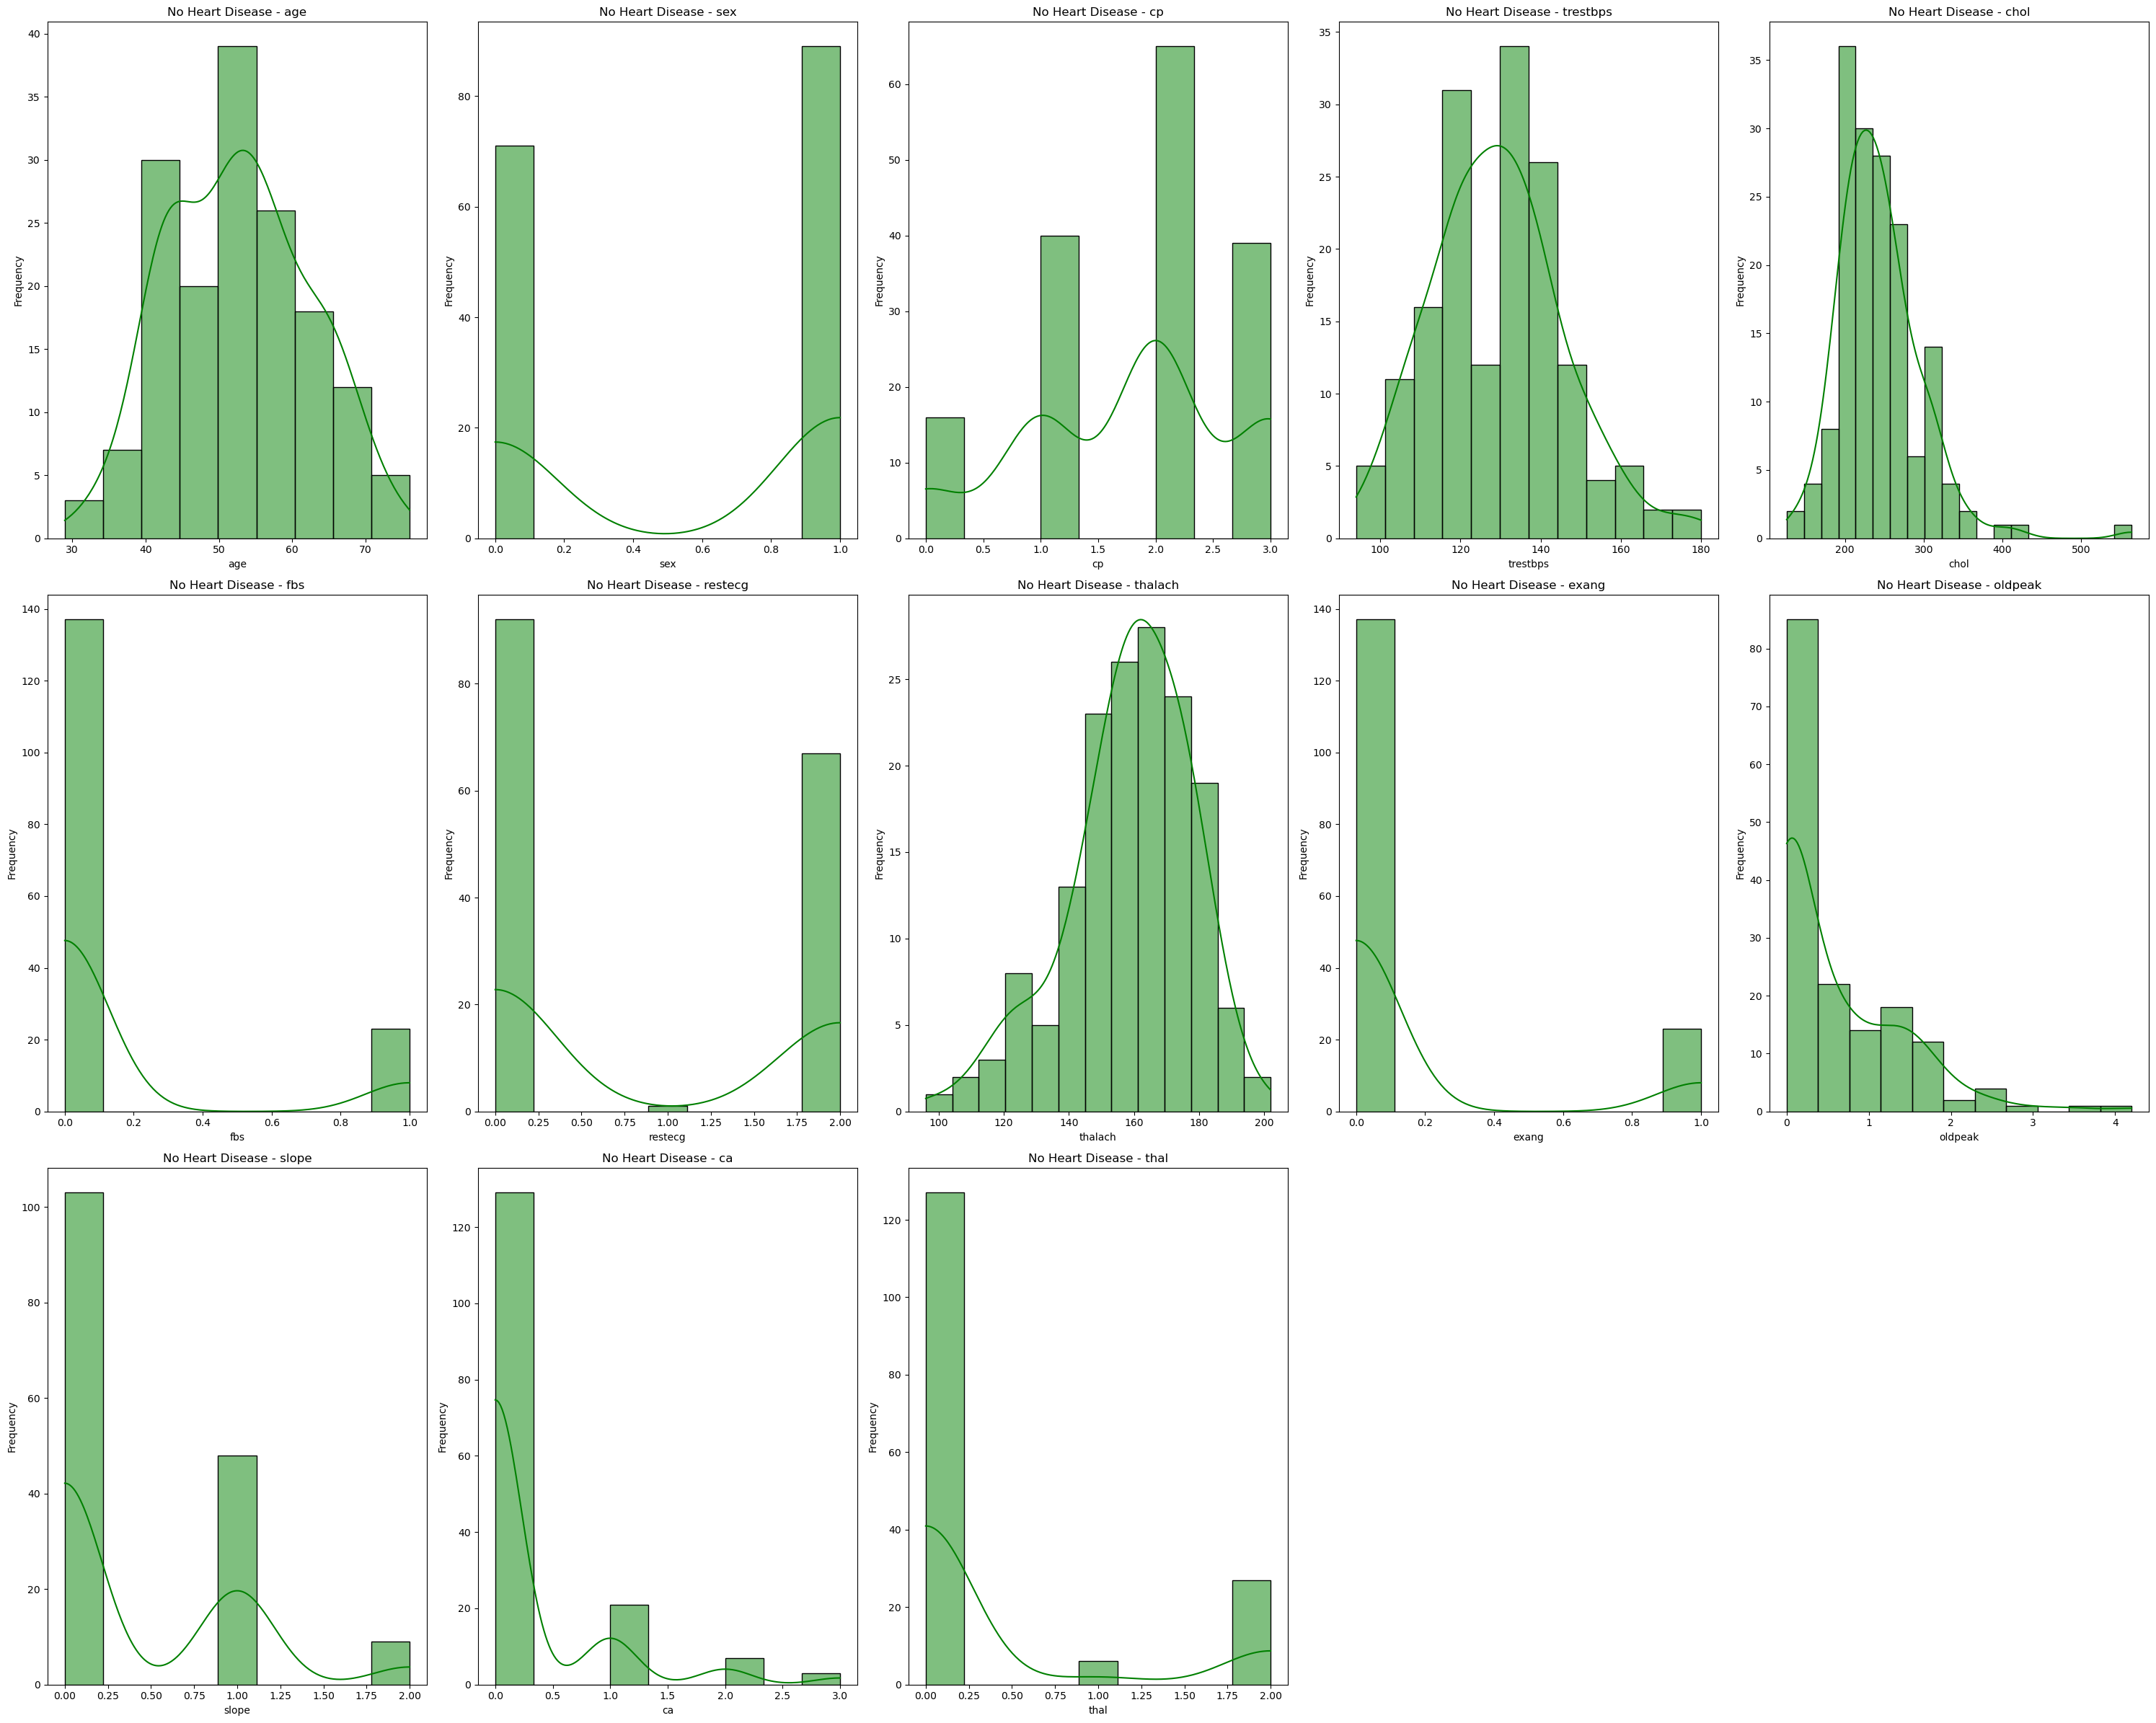
\includegraphics[width=1\linewidth]{images/no_heart_distribution.png}
    \caption{Distribution of patients healthy patients (without heart disease)}
    \label{fig:no_heart_distribution}
\end{figure}

\begin{figure}[!htb]
    \centering
    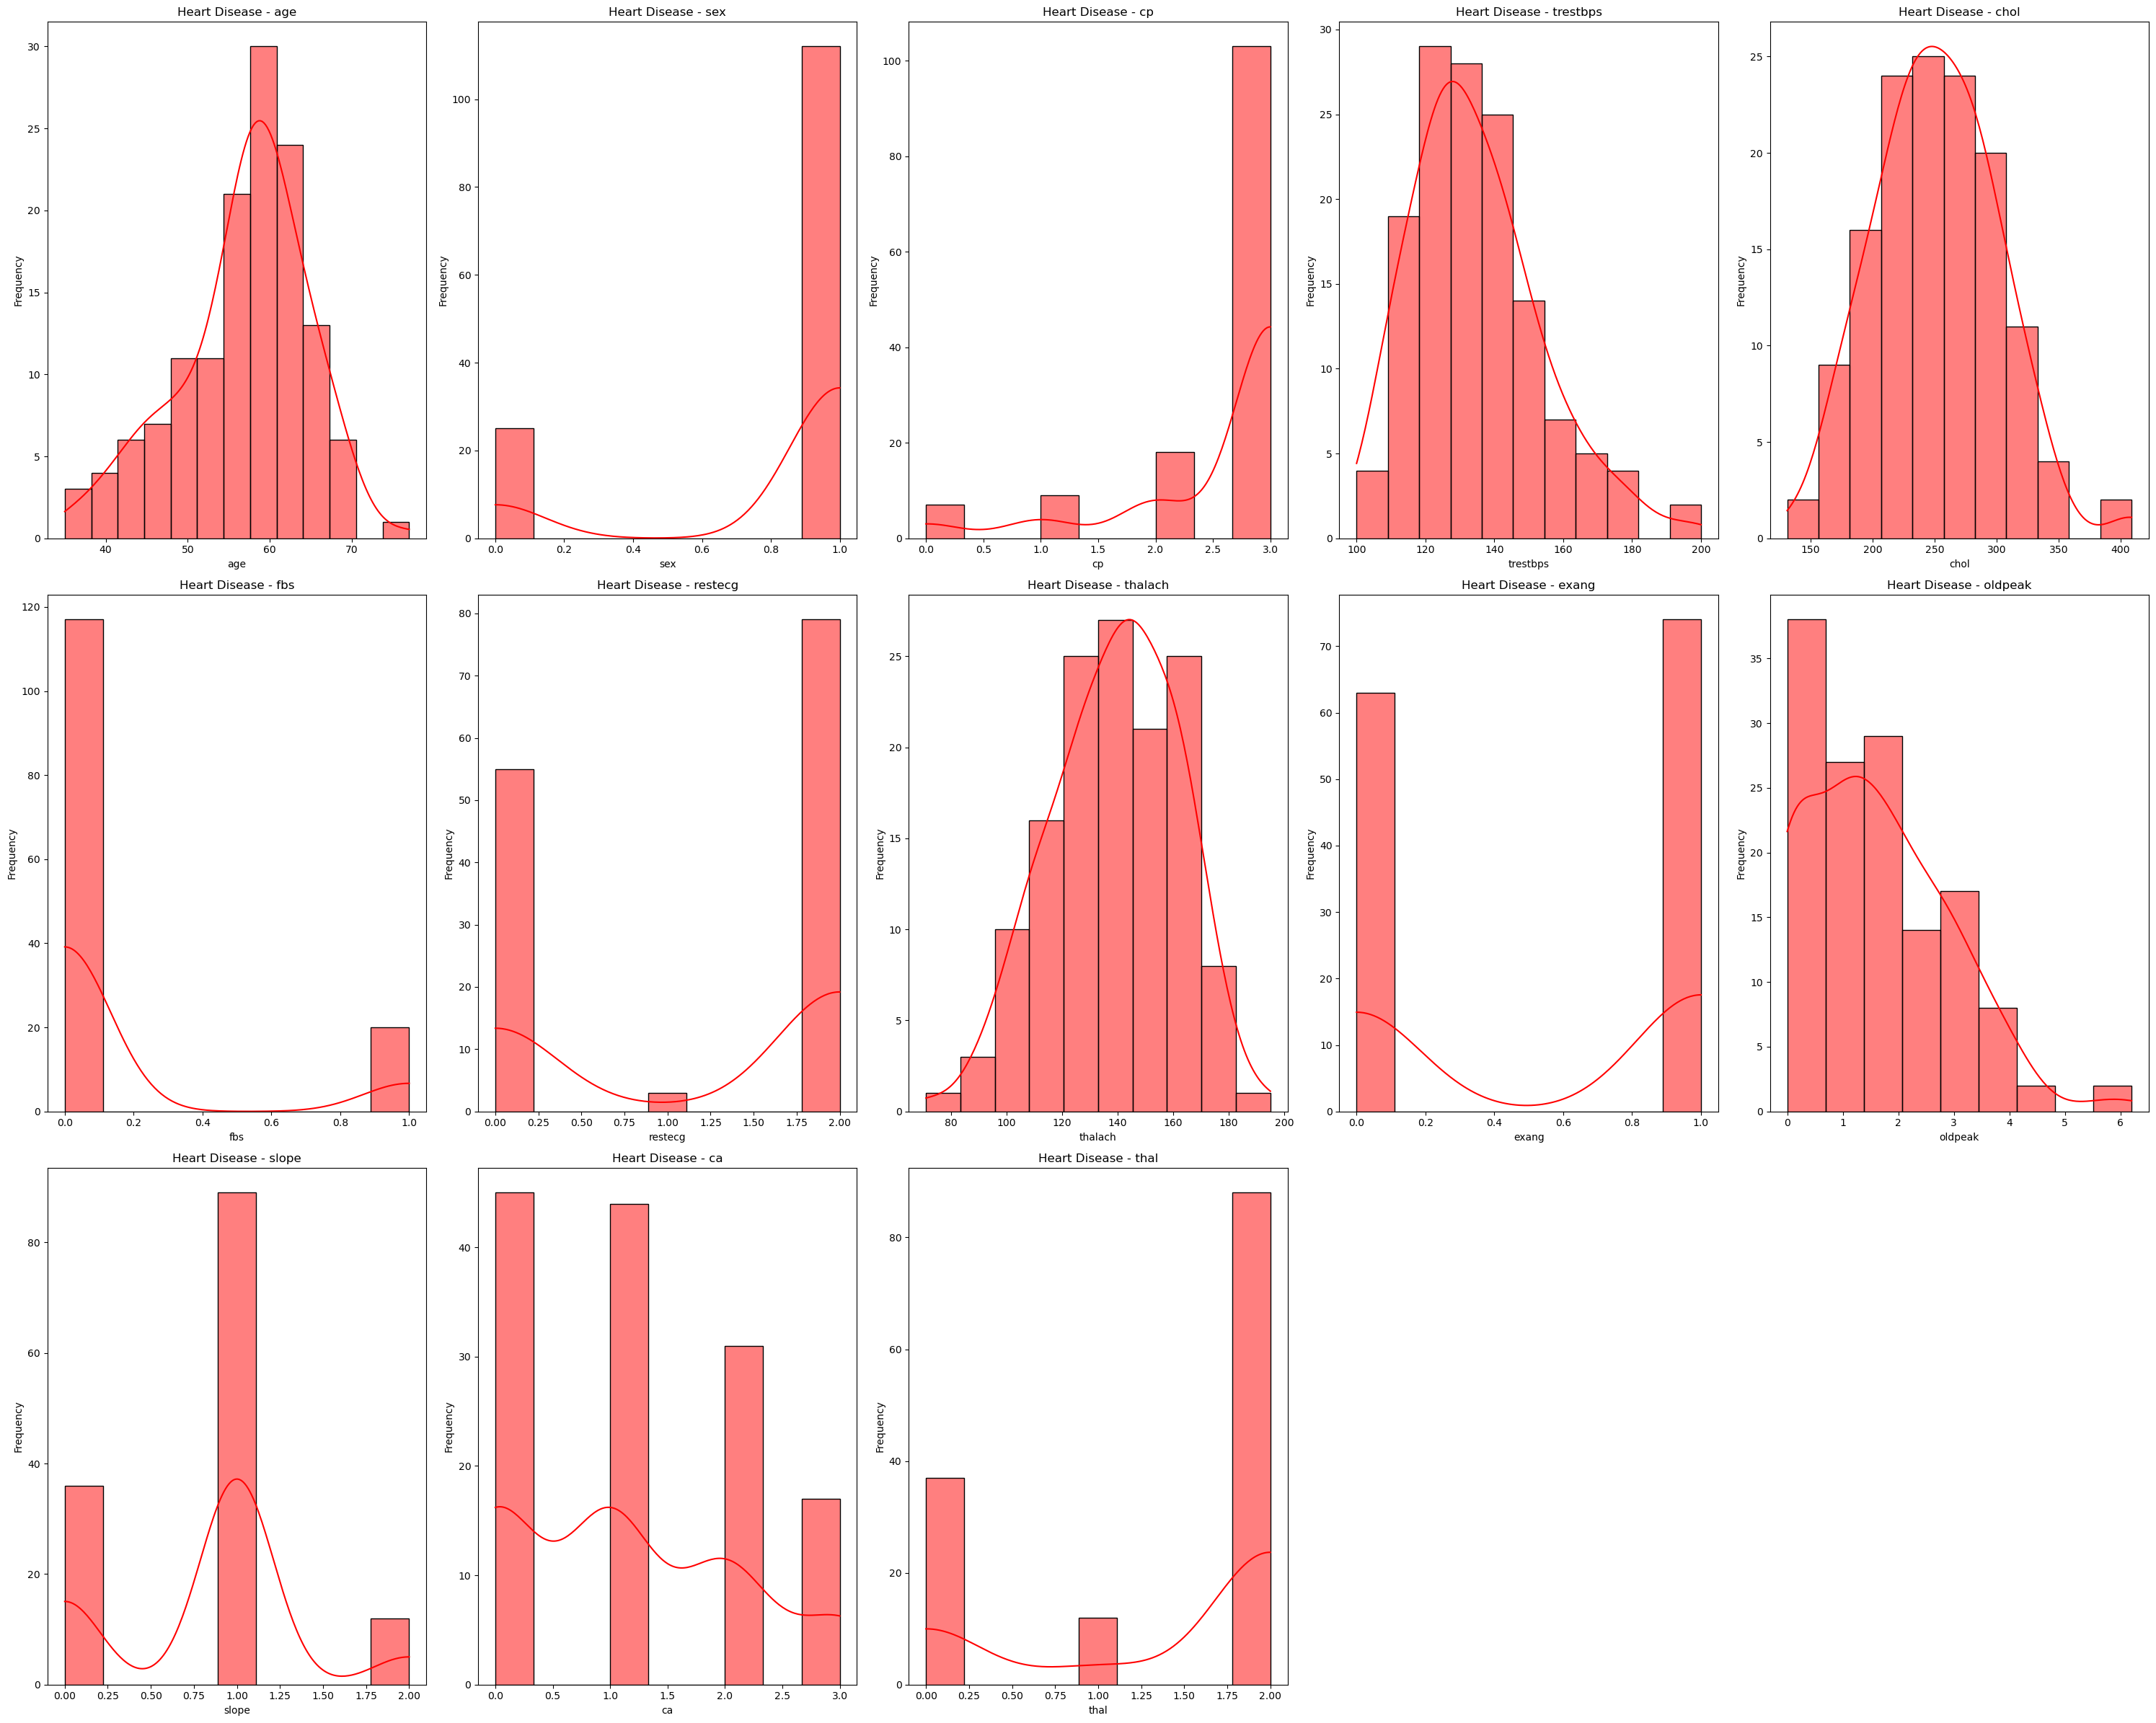
\includegraphics[width=1\linewidth]{images/heart_distribution.png}
    \caption{Distribution of patients with heart disease}
    \label{fig:heart_distribution}
\end{figure}

\begin{enumerate}
    \item Age Distribution:
 Patients with heart disease show a clear peak in the 60–70-year age range, reflecting a higher prevalence of the condition in older individuals. In contrast, patients without heart disease display a more uniform age distribution, indicating less dependency on age in this group.

    \item Sex Distribution:
 The group with heart disease has a significantly higher proportion of male patients compared to the group without heart disease. This aligns with the well-documented higher risk of heart disease in men.

    \item Chest Pain Type (CP) Distribution:
Among patients with heart disease, the distribution of chest pain types has a high peak at the highest value of CP. This suggests that this specific type of chest pain is strongly associated with the presence of heart disease. In comparison, the no heart disease group shows a more uniform distribution across CP types.

    \item Resting Blood Pressure (Trestbps) Distribution:
The heart disease group exhibits a slightly more right-skewed distribution of resting blood pressure values.

    \item Serum Cholesterol (Chol) Distribution:
Even though the cholesterol levels among patients with heart disease tend to be right-skewed, with higher values compared to those without heart disease, in our dataset both the groups of diseased and healthy patients have an even distribution of this measure.

    \item Slope of the Peak Exercise ST Segment Distribution:
 The slope distribution in the heart disease group is unimodal with a peak at the flat category of slope. A flat or horizontal ST segment depression during exercise stress testing is often considered abnormal. It suggests myocardial ischemia, which occurs when there is insufficient blood flow to the heart muscle during stress, typically due to atherosclerotic coronary artery disease. In contrast, the no heart disease group have the most frequency in the upsloping category suggesting that they are healthy individuals. 
\end{enumerate}

These differences in attribute distributions between the two groups highlight the importance of factors such as age, sex, chest pain type, blood pressure, cholesterol levels, and exercise-induced ST segment slope in identifying and assessing the risk of heart disease. Understanding these patterns not only aids in distinguishing between individuals with and without the condition but also provides a foundation for more targeted diagnostic and preventive approaches.

\subsection{Correlation Matrix Insights} 
The correlation matrix present in Fig. 13 reveals important relationships between the attributes and the target variable. 
\begin{figure}[H]
    \centering
    \includegraphics[width=1\linewidth]{images/matriz_correçacao.png}
    \caption{Correlation Matrix}
    \label{fig:enter-label}
\end{figure}

These can help in the process of feature selection and model development for heart disease prediction:
\begin{itemize}
    \item Age has a moderate positive correlation (0.23) with the target, indicating that the likelihood of heart disease increases with age.
    \item Sex also shows a moderate positive correlation (0.28) with the target, suggesting that being male is associated with a higher risk of heart disease.
    \item Chest Pain Type (CP) has a moderately strong positive correlation (0.41), implying that specific chest pain types are more indicative of heart disease.
    \item Thalach (Maximum Heart Rate Achieved) shows a moderately strong negative correlation (-0.42), indicating that lower maximum heart rates are associated with a higher risk of heart disease.
    \item Exercise-Induced Angina (Exang) and Oldpeak (ST Depression) both have a moderately strong positive correlation (0.42) with the target, highlighting their significance in heart disease prediction.
    \item Ca (Number of Major Vessels Colored by Fluoroscopy) has a positive correlation (0.46), making it one of the stronger predictors of heart disease.
    \item Thal (Thalassemia) demonstrates the strongest positive correlation (0.52) with the target, indicating its significant role in predicting heart disease.
\end{itemize}

Additional Observations:

\begin{itemize}
    \item Attributes such as Chol (Serum Cholesterol) and Trestbps (Resting Blood Pressure) have low positive correlations (0.08 and 0.15, respectively), suggesting limited predictive power when considered individually.
    \item Fbs (Fasting Blood Sugar) shows a near-zero correlation (0.00), implying minimal influence on heart disease prediction in this dataset.
    \item Several attributes, including Slope, Restecg, and Oldpeak, exhibit moderate correlations with one another (e.g., Slope and Oldpeak: 0.58), indicating potential interactions that could enhance predictive modeling.
\end{itemize}

While some attributes show strong linear relationships with the target, many exhibit low correlations (< 0.3). This suggests that more complex modeling techniques may be required to capture non-linear relationships and interactions among the attributes for accurate heart disease prediction.
\section{Implementation details}
Before applying the models, it was essential to prepare the data through standardization and splitting into training and testing sets. Standardization ensures that all features have a mean of 0 and a standard deviation of 1, making the data suitable for algorithms sensitive to feature scaling. This was achieved using the StandardScaler\cite{StandardScaler}:
\begin{python}
# Standardize
scaler = StandardScaler()
X = scaler.fit_transform(X)

# Split Data
X_train, X_test, y_train, y_test = 
        train_test_split(X, y, stratify=y, 
                    test_size=0.2, random_state=21)
\end{python}
The train-test split was performed with an 80-20 ratio, stratifying by the target variable to maintain class balance in both sets. This step ensures fair evaluation of the models on unseen data.

%\newline
%\bigskip
%\newline
%\bigskip
%\newline
%\bigskip\newline
%\bigskip
\subsection{Model Development Workflow}
For each of the \acrshort{ml} models applied in this study, the following sequence of steps was used:
\begin{enumerate}
\item Base Model:
The initial model was applied using default hyperparameters. This model serves as a baseline for comparison with subsequent models. By establishing baseline metrics such as Accuracy, F1 score, Precision, and Recall, we can evaluate the impact of further optimizations.

\item Hyperparameter Tuned Model:
To enhance the model’s performance, we focused on optimizing the hyperparameters, which balances regularization strength and data fitting. Using RandomizedSearchCV\cite{RandomizedSearchCV}:
\begin{python}
model = RandomizedSearchCV(
        hypertuned_model, 
        hyperparameters, 
        scoring="accuracy", 
        n_iter=n_iter, 
        random_state=42,  
        verbose=1
    )
\end{python}

\begin{itemize} \item Scoring Metric: Accuracy was used to evaluate the effectiveness of each parameter combination. \item Number of Iterations (n\_iter): Limited to ensure efficient exploration of the hyperparameter space. \end{itemize}

\item K-Fold Cross-Validation Model:
The optimized hyperparameter-tuned model was further evaluated using dynamic K-Fold Cross-Validation. Instead of fixing the number of folds at 5, the algorithm iteratively evaluated the model over k (in our case 10) folds, selecting the fold with the highest accuracy as the best estimator. This approach ensures that the model's performance generalizes well across different subsets of the data and identifies the optimal fold for the most reliable estimator.
\end{enumerate}

\section{Results}
\subsection{Logistic Regression}
We applied logistic regression using three approaches: the Base Model, the Hyper-Parameter Selection Model, and K-Fold Cross-Validation on the Hyper-Parameter Selection Model. 

\subsubsection{Base Model}
Table \ref{tab:tab1} presents the hyperparameters selected for the base model.

\begin{table}[ht]
    \centering
    \caption{Base hyperparameters in Logistic Regression} 
    \begin{tabular}{||c c c c c||} 
     \hline
     C & class\_weight & max\_iter & penalty & solver \\ [0.5ex] 
     \hline\hline
     1.0 & None & 100 & l2 & lbfgs \\ 
    \hline
    \end{tabular}
    \label{tab:tab1}
\end{table}

In the base Logistic Regression model, the following hyperparameters were used:

\begin{itemize}
    \item C: Set to 1.0, this hyperparameter controls the trade-off between model complexity and training accuracy. It is the inverse of the regularization strength. A smaller value increases regularization, reducing the influence of less important features, while a larger value prioritizes fitting the training data over regularization.
    \item class\_weight: Set to None, meaning no explicit balancing was applied to account for class imbalances.
    \item max\_iter: Defined as 100, this represents the maximum number of iterations the solver is allowed to perform to converge to a solution.
    \item penalty: The l2 regularization was used, which minimizes the sum of the squared coefficients to penalize large values and reduce overfitting.
    \item solver: The solver was set to lbfgs, an efficient optimization algorithm commonly used for logistic regression with small to medium-sized datasets.
\end{itemize}

The results for the Base Model application are:

\begin{figure}[H]
    \centering
    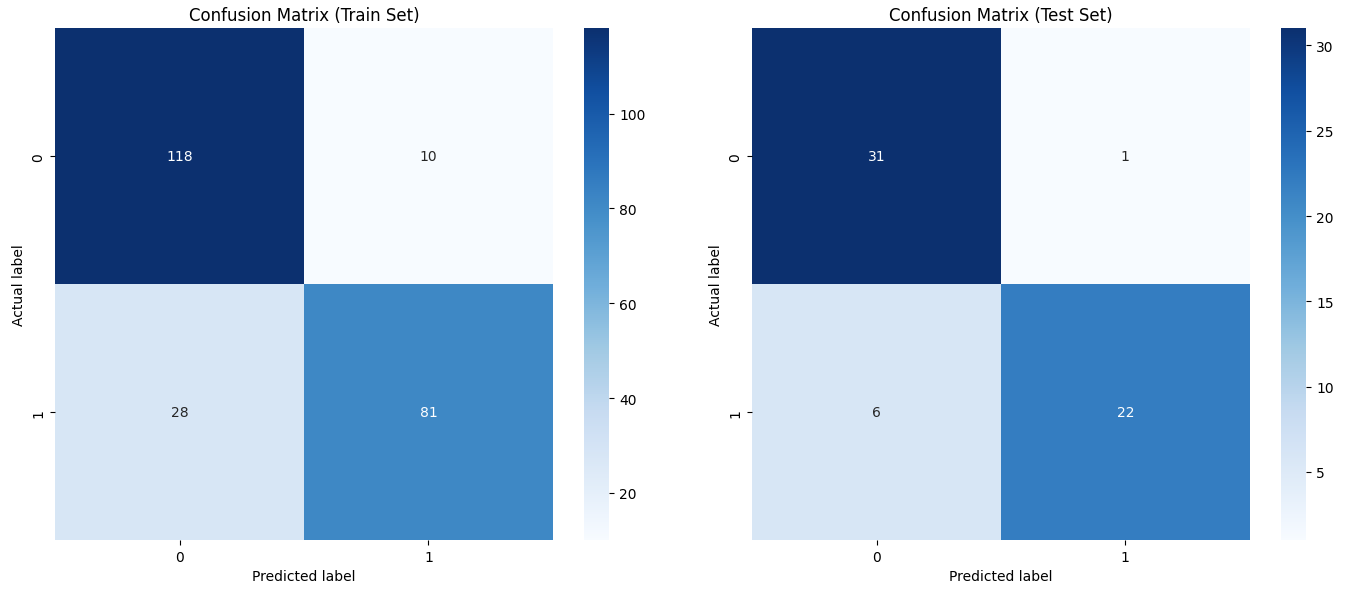
\includegraphics[width=1\linewidth]{images/confusion_matrix_lg_reg_base.png}
    \caption{Confusion Matrix}
    \label{fig:enter-label}
\end{figure}
\begin{figure}[H]
    \centering
    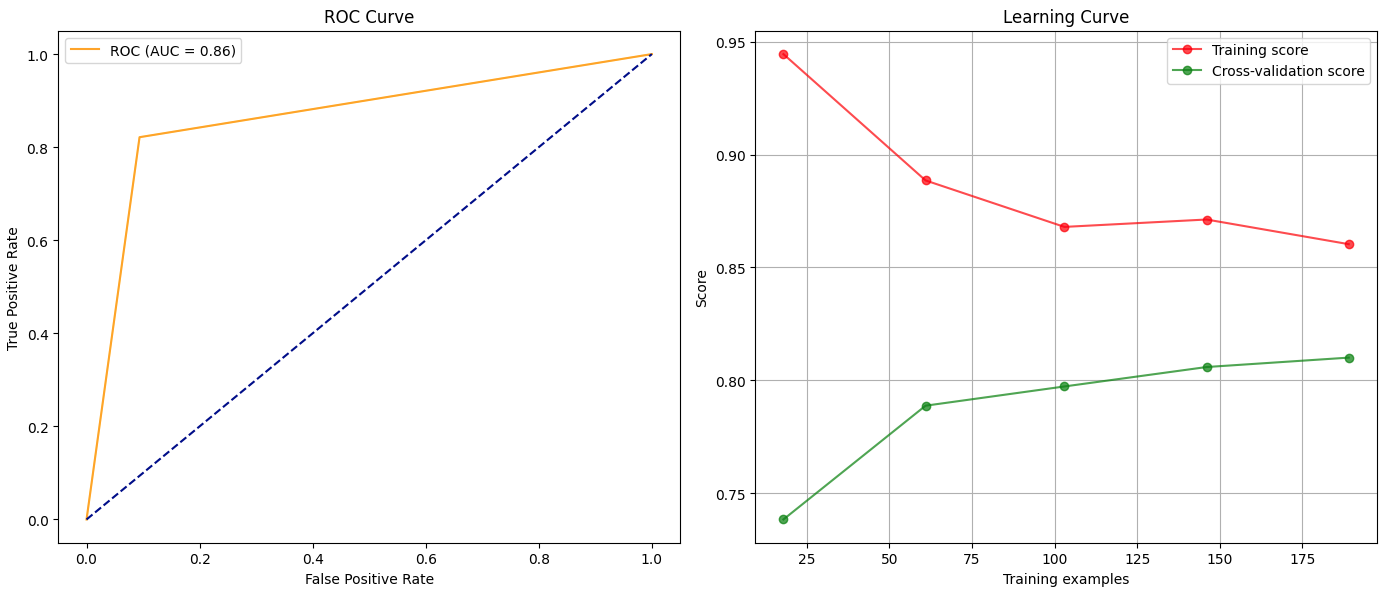
\includegraphics[width=1\linewidth]{images/roc_learning_logreg_base.png}
    \caption{ROC Curve and Learning Curve}%
    \label{fig:enter-label}
\end{figure}

\subsubsection{Hyper-Parameter Selection Model}

Next, we performed a search for the optimal value of C. The choice of C plays a critical role in determining the balance between fitting the training data and generalization. A value that is too small may lead to underfitting, while a very large value could lead to overfitting.

To find the best value for C, we employed RandomizedSearchCV with a range of values:
\begin{equation}
C \in \{0.001, 0.01, 0.1, 1, 10, 100\}
\end{equation}


\begin{table}[ht]
    \centering
    \caption{Best hyperparameters in Logistic Regression} 
    \begin{tabular}{||c c c c c||} 
     \hline
     C & class\_weight & max\_iter & penalty & solver \\ [0.5ex] 
     \hline\hline
     0.01 & None & 100 & l2 & lbfgs \\ 
    \hline
    \end{tabular}
    \label{tab:tab2}
\end{table}


The results for the Hyper-Parameter Selection Model are:
\begin{figure}[H]
    \centering
    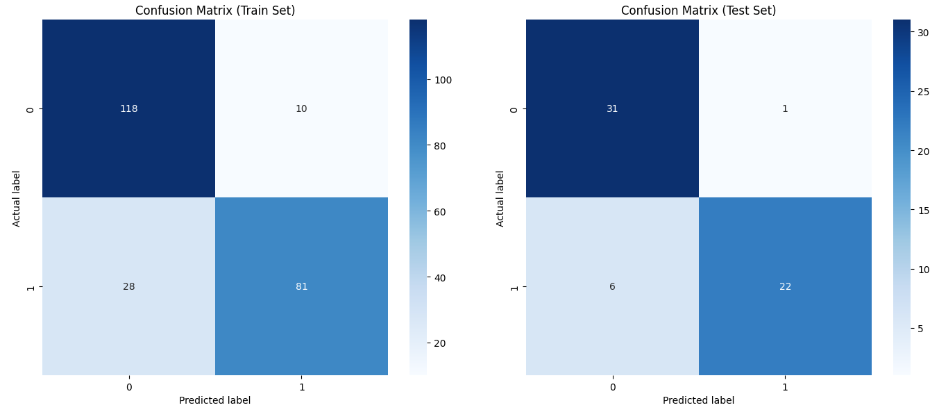
\includegraphics[width=1\linewidth]{images/confusion_matrix_lg_reg_search.png}
    \caption{Confusion Matrix}
    \label{fig:enter-label}
\end{figure}
\begin{figure}[H]
    \centering
    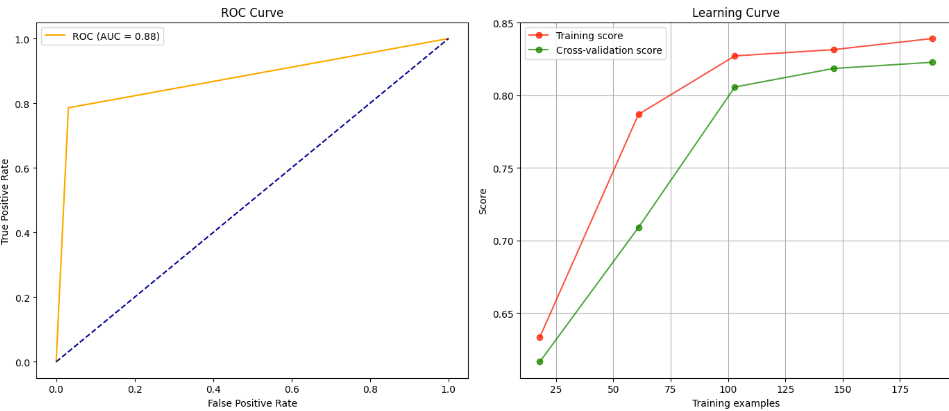
\includegraphics[width=1\linewidth]{images/roc_learning_logreg_search.png}
    \caption{ROC Curve and Learning Curve}%
    \label{fig:enter-label}
\end{figure}


\subsubsection{K-Fold Cross-Validation Model}

To evaluate the model's robustness and minimize the risk of overfitting, we applied K-Fold Cross-Validation. 

The results of the K-Fold Cross-Validation are shown in Figure \ref{fig:kfold_logReg}. Each fold's accuracy score is visualized, allowing us to identify the fold with the highest accuracy. In this case, the fold with the best performance was Fold 8, which achieved the highest accuracy.

\begin{figure}[H] \centering 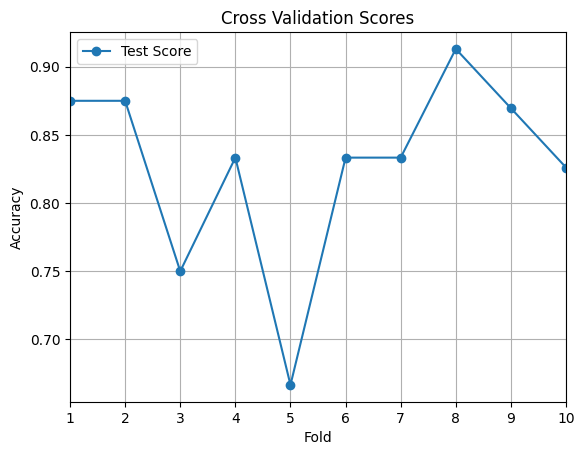
\includegraphics[width=0.75\linewidth]{images/k_fold_cross_log_reg.png} \caption{Accuracy Scores Across K-Folds} \label{fig:kfold_logReg} \end{figure}

Based on this result, the model corresponding to the best-performing fold (Fold 8) was selected and retrained on the entire training dataset. This ensures that the final model leverages all available training data while incorporating the insights gained from the cross-validation process.
The results for the K-Fold Cross-Validation Model are:

\begin{figure}[H]
    \centering
    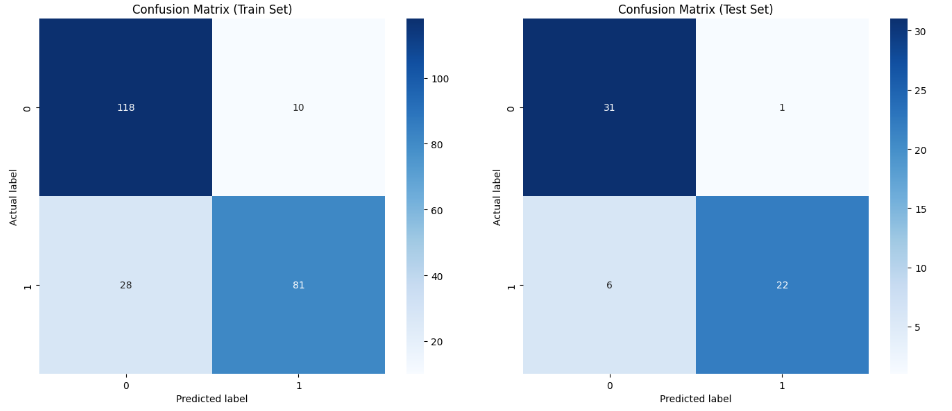
\includegraphics[width=1\linewidth]{images/confusion_matrix_lg_reg_kfold.png}
    \caption{Confusion Matrix}
    \label{fig:enter-label}
\end{figure}
\begin{figure}[H]
    \centering
    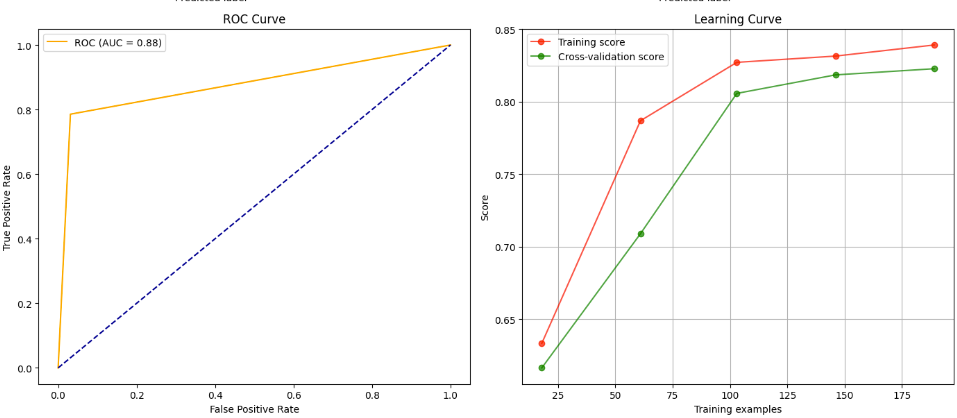
\includegraphics[width=1\linewidth]{images/roc_learning_logreg_kfold.png}
    \caption{ROC Curve and Learning Curve}%
    \label{fig:enter-label}
\end{figure}

\begin{figure}[H]
    \centering
    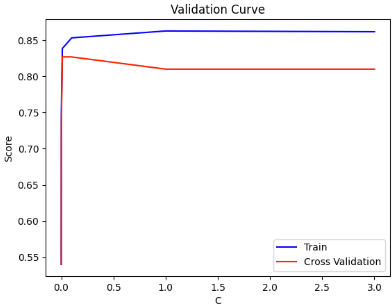
\includegraphics[width=0.75\linewidth]{images/validation_curve_log_reg.png}
    \caption{Validation Curve}
    \label{fig:ValidationCurveLogReg}
\end{figure}

\subsubsection{Conclusions}
Observing the confusion matrices, we can conclude that the number of incorrectly classified examples, the sum of \acrfull{FP} and \acrfull{FN}, is very low compared to the number of correctly classified examples, sum of \acrfull{TP} with \acrfull{TN}. Therefore, we can consider the model accurate.

The higher the AUC score, the better the performance of a classifier for a given task. Therefore, through the ROC Curve graphs, we can say that the classifier performed well because the AUC value is 0.86/0.88. It has good predictive power.

In Fig \ref{fig:ValidationCurveLogReg}, we observe that C values in the range between 0 and 3 are suitable, with the best performance concentrated in the interval from 0 to 2. After a value close to 0, both training accuracy and cross-validation accuracy stabilize, with training scores averaging around 0.85 and cross-validation scores around 0.81.

The differences between training and validation scores are minimal, indicating that the model achieves a good balance between bias and variance. This behavior suggests that variations in the C parameter within this range have an insignificant impact on the overall performance of the model, making it robust for this interval of values.

\begin{table}[H]
    \centering
    \caption{Classification - All Model} 
    \begin{tabular}{||c| c c c c||} 
     \hline
     & Accuracy & F1 Score & Recall & Precision \\
     \hline\hline
     Base Model & 0.867 & 0.852 & 0.821 & 0.885 \\
     \hline
    Hyper-Parameter & 0.883 & 0.863 & 0.79 & 0.957 \\ 
    \hline
    K-Fold & 0.883 & 0.863 & 0.79 & 0.957 \\ 
    \hline
    \end{tabular}
    \label{tab:tab_LogReg}
\end{table}

By examining Table \ref{tab:tab_LogReg}, we observe that the Accuracy and F1 Score for the Hyper-Parameter Selection Model and K-Fold Cross-Validation Model are identical, both slightly outperforming the Base Model. While the Base Model achieves a good Precision (0.885), the Hyper-Parameter and K-Fold models significantly improve it to 0.957, indicating a better ability to correctly identify true positive cases among all positive predictions.

However, the Recall (or Sensibility) is slightly lower for the Hyper-Parameter and K-Fold models (0.79) compared to the Base Model (0.821). This indicates that the Base Model is slightly better at identifying the real positive cases, but at the cost of reduced Precision.

In this context, even though it is critical to minimize false negatives because missing a cancer diagnosis can have more severe consequences than giving a false diagnosis, the Hyper-Parameter Selection and K-Fold models are preferable because they have a much higher Precision and their differences in Recall are minimal compared to the Base-Model.

%%%%%%%%%%%%%%%%%%%%%%%%%%%%%%%% SVC %%%%%%%%%%%%%%%%%%%%%%%%%
\bigskip
\subsection{Support Vector Machine}

We applied SVC using three approaches: the Base Model, the Hyper-Parameter Selection Model, and K-Fold Cross-Validation on the Hyper-Parameter Selection Model. 

\subsubsection{Base Model}
Table \ref{tab:tab1_svc} presents the parameters selected for the base model.

\begin{table}[ht]
    \centering
    \caption{Base parameters in SVC} 
    \begin{tabular}{||c c c c c||} 
     \hline
     C & class\_weight & max\_iter & gamma & kernel \\ [0.5ex] 
     \hline\hline
     1.0 & None & 100 & scale & rbf \\ 
    \hline
    \end{tabular}
    \label{tab:tab1_svc}
\end{table}

In the base SVC model, the following parameters were used:

\begin{itemize}
    \item C: Set to 1.0, this hyperparameter controls the trade-off between model complexity and training accuracy. It is the inverse of the regularization strength. A smaller value increases regularization, reducing the influence of less important features, while a larger value prioritizes fitting the training data over regularization.
    \item class\_weight: Set to None, meaning no explicit class balancing was applied. This can lead to biased results in imbalanced datasets. 
    \item max\_iter: Defined as 100, representing the maximum number of iterations the solver is allowed to perform to reach convergence. If the solver does not converge within 100 iterations, the process stops. 
    \item gamma: Set to "scale," which automatically calculates the gamma parameter as \[
    \gamma = \frac{1}{\text{number of features}}
    \] This controls the influence of a single training example, with higher values leading to tighter decision boundaries.
    \item kernel: Set to rbf (Radial Basis Function), which is a popular kernel function in SVC models. It allows the model to capture non-linear relationships between features by mapping the data into a higher-dimensional space.
\end{itemize}

The results for the Base Model application are:

\begin{figure}[H]
    \centering
    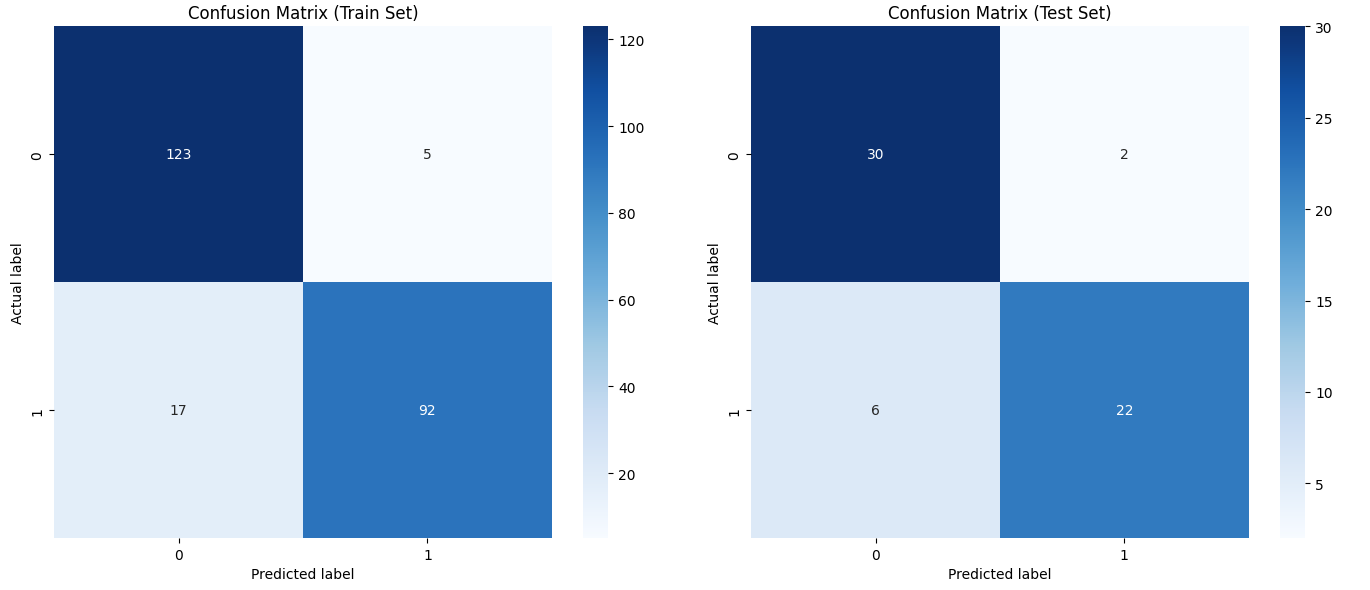
\includegraphics[width=1\linewidth]{images/confusion_matrix_svc_base.png}
    \caption{Confusion Matrix}
    \label{fig:enter-label}
\end{figure}
\begin{figure}[H]
    \centering
    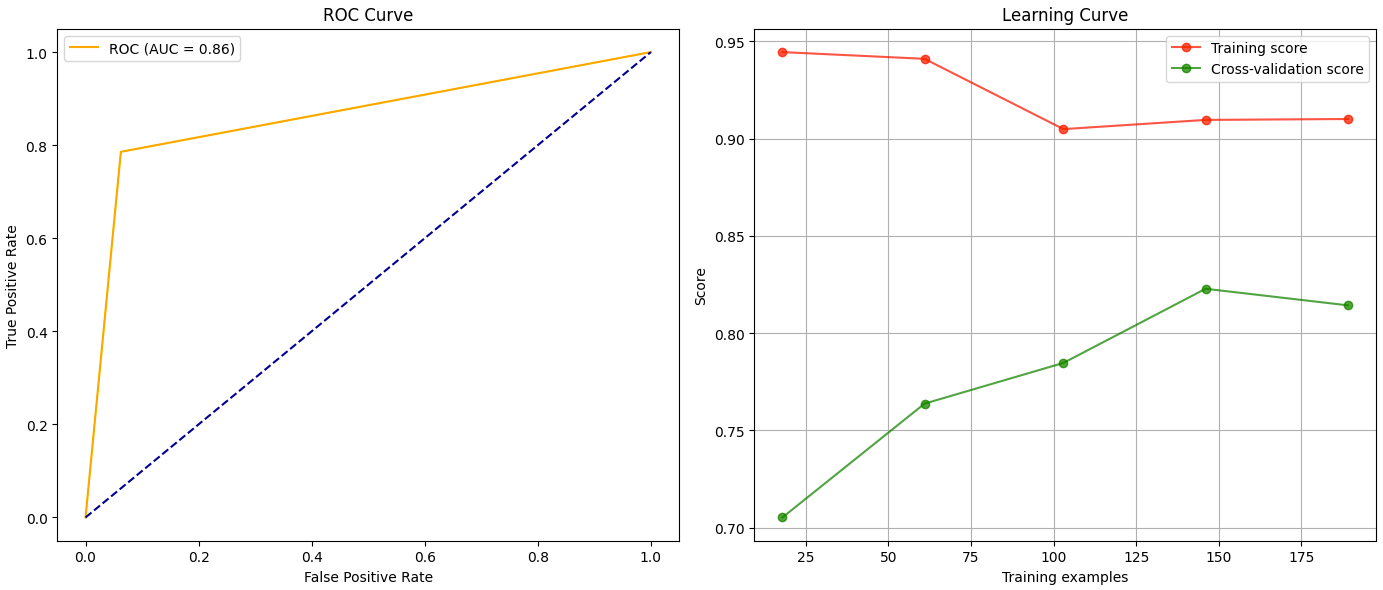
\includegraphics[width=1\linewidth]{images/roc_learning_svc_base.png}
    \caption{ROC Curve and Learning Curve}%
    \label{fig:enter-label}
\end{figure}

\subsubsection{Hyper-Parameter Selection Model}

Next, we performed a search for the optimal values of C, the regularization parameter, and gamma, the kernel coefficient. Both parameters play a critical role in determining the model's performance.

\begin{itemize}
    \item \textbf{C} controls the trade-off between fitting the training data and applying regularization. A smaller value of C increases regularization, which can lead to underfitting, while a larger value reduces regularization, potentially leading to overfitting.
    \item \textbf{gamma} defines how far the influence of a single training example reaches. Higher values of gamma result in tighter decision boundaries, which can capture more complex patterns but may also lead to overfitting. Lower values lead to smoother decision boundaries and better generalization.
    \item \textbf{kernel}: The kernel function is used to map the original data into a higher-dimensional space, where a linear decision boundary can separate the data more effectively. We experimented with different kernel functions:
\begin{itemize}
    \item rbf (Radial Basis Function): This is the most commonly used kernel, which computes the similarity between points using the distance between them, allowing for non-linear decision boundaries.
    \item linear: This kernel is used when the data is linearly separable, and it directly applies a linear decision boundary.
    \item poly (Polynomial): This kernel allows for decision boundaries based on polynomial functions of the input features, making it suitable for datasets with more complex, but still polynomially separable, relationships.
\end{itemize}
\end{itemize}

To find the optimal values for these parameters, we employed RandomizedSearchCV with the following ranges:
\begin{equation}
C \in \{0.01, 0.1, 1, 10, 100\}
\end{equation}
\begin{equation}
gamma \in \{10, 1, 0.1, 0.01, 0.001\}
\end{equation}
\begin{equation}
kernel \in \{'rbf','linear','poly'\}
\end{equation}


\begin{table}[ht]
    \centering
    \caption{Best parameters in SVC} 
    \begin{tabular}{||c c c c c||} 
     \hline
     C & class\_weight & max\_iter & gamma & kernel \\ [0.5ex] 
     \hline\hline
     0.01 & None & 100 & 1 & linear\\ 
    \hline
    \end{tabular}
    \label{tab:tab2_svc}
\end{table}

The results for the Hyper-Parameter Selection Model are:
\begin{figure}[H]
    \centering
    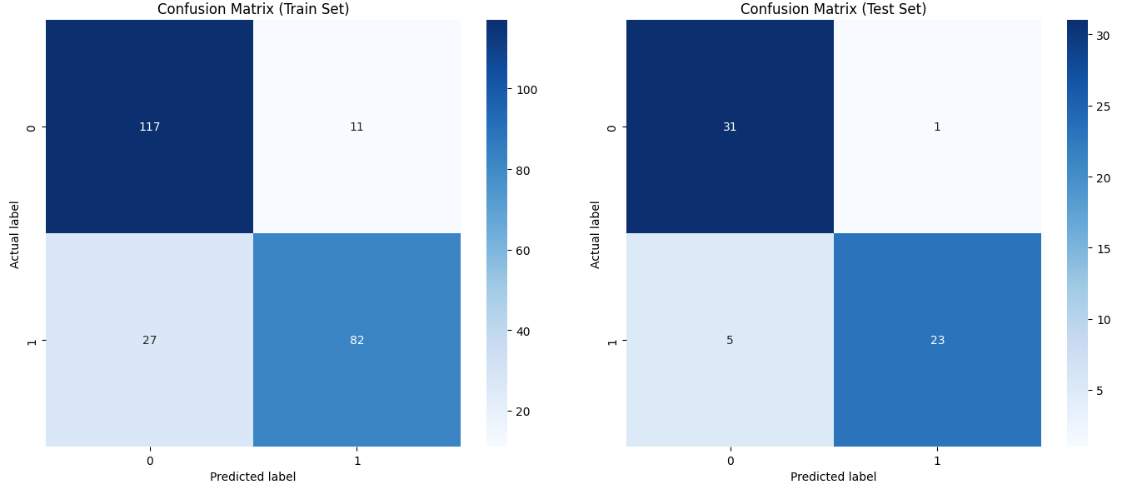
\includegraphics[width=1\linewidth]{images/confusion_matrix_svc_search.png}
    \caption{Confusion Matrix}
    \label{fig:enter-label}
\end{figure}
\begin{figure}[H]
    \centering
    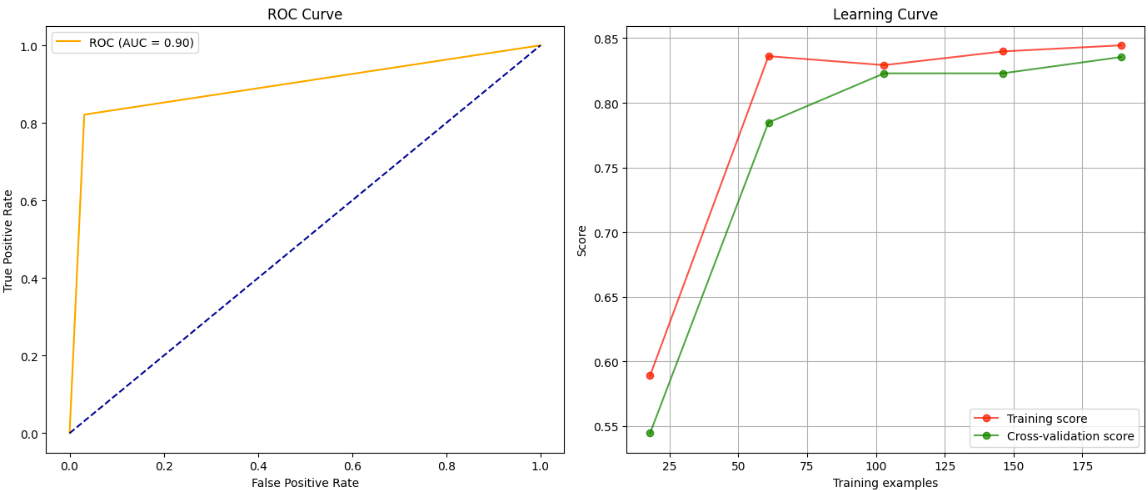
\includegraphics[width=1\linewidth]{images/roc_learning_svc_search.png}
    \caption{ROC Curve and Learning Curve}%
    \label{fig:enter-label}
\end{figure}


\subsubsection{K-Fold Cross-Validation Model}

To evaluate the model's robustness and minimize the risk of overfitting, we applied K-Fold Cross-Validation. 

The results of the K-Fold Cross-Validation are shown in Figure \ref{fig:k_fold_cross_svc.png}. Each fold's accuracy score is visualized, allowing us to identify the fold with the highest accuracy. In this case, the fold with the best performance was Fold 2, which achieved the highest accuracy.

\begin{figure}[H] \centering 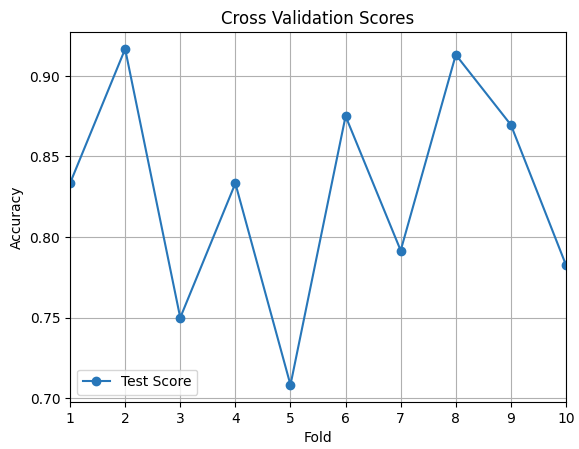
\includegraphics[width=0.75\linewidth]{images/k_fold_cross_svc.png} \caption{Accuracy Scores Across K-Folds} \label{fig:k_fold_cross_svc.png} \end{figure}

Based on this result, the model corresponding to the best-performing fold (Fold 2) was selected and retrained on the entire training dataset. This ensures that the final model leverages all available training data while incorporating the insights gained from the cross-validation process.

The results for the K-Fold Cross-Validation Model are:

\begin{figure}[H]
    \centering
    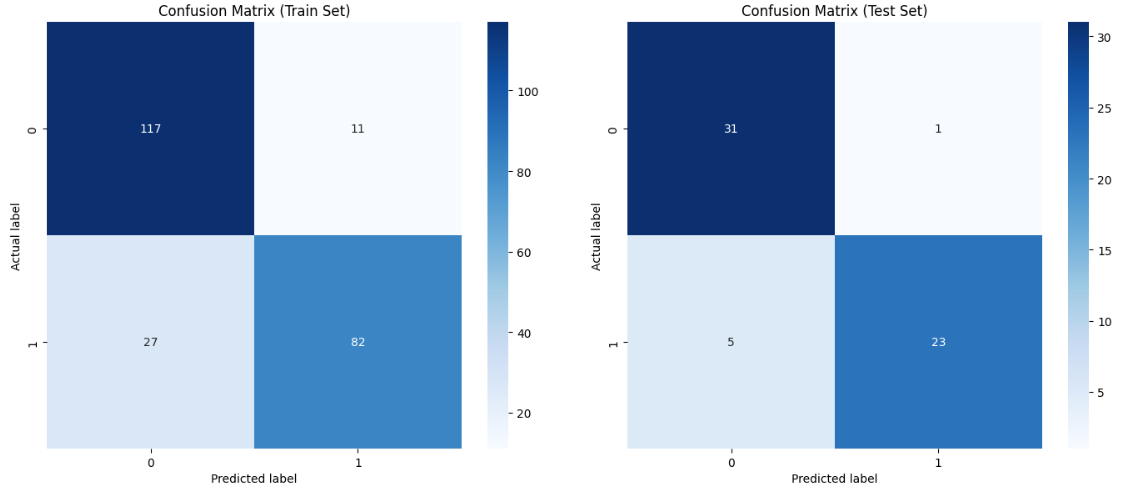
\includegraphics[width=1\linewidth]{images/confusion_matrix_svc_kfold.png}
    \caption{Confusion Matrix}
    \label{fig:enter-label}
\end{figure}
\begin{figure}[H]
    \centering
    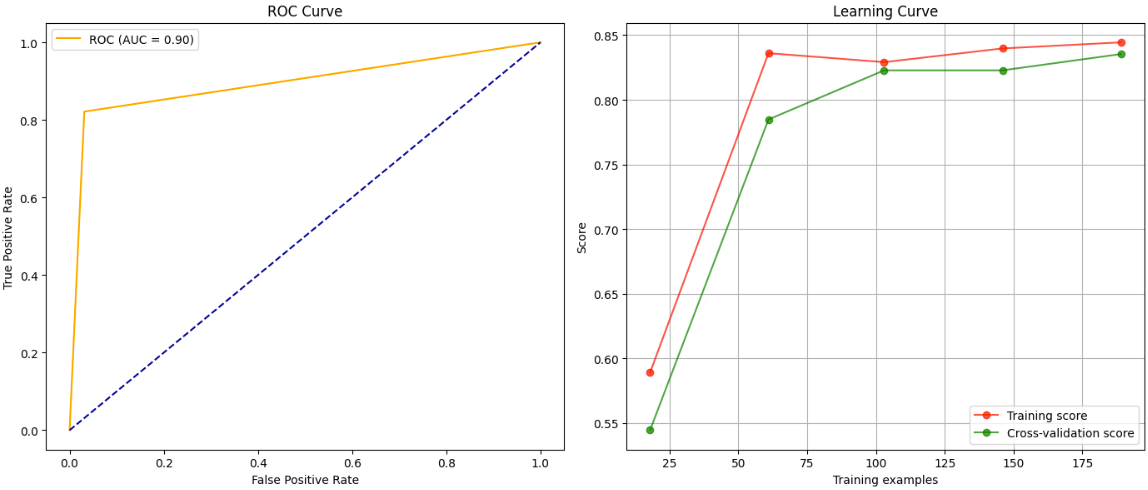
\includegraphics[width=1\linewidth]{images/roc_learning_svc_kfold.png}
    \caption{ROC Curve and Learning Curve}%
    \label{fig:enter-label}
\end{figure}

\begin{figure}[H]
    \centering
    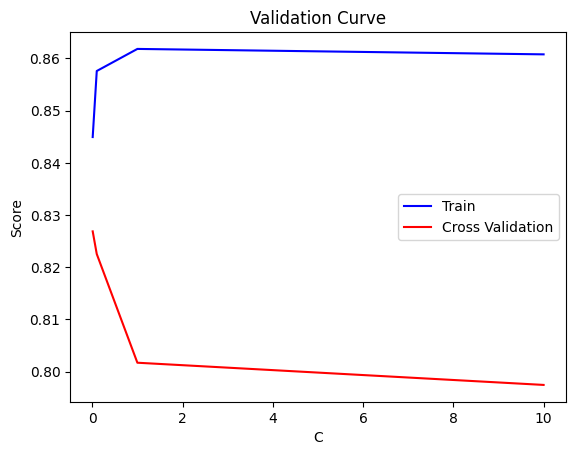
\includegraphics[width=0.75\linewidth]{images/validation_curve_c_svc.png}
    \caption{Validation Curve}
    \label{fig:ValidationCurveC_SVC}
\end{figure}
\begin{figure}[H]
    \centering
    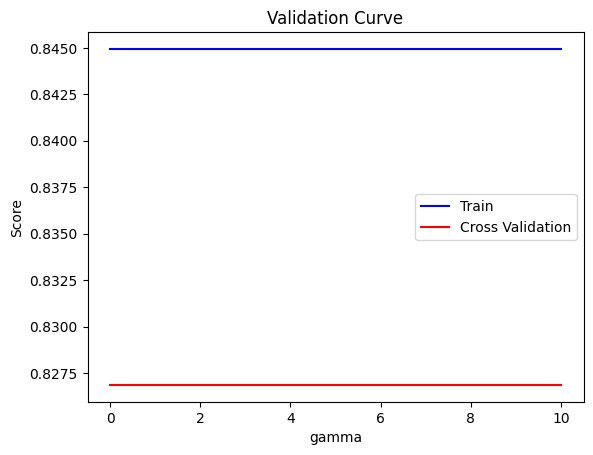
\includegraphics[width=0.75\linewidth]{images/validation_curve_gamma_svc.png}
    \caption{Validation Curve}
    \label{fig:ValidationCurveGamma_SVC}
\end{figure}

\subsubsection{Conclusions}
As observed previously in the Logistic Regression results, the confusion matrices for the Support Vector Classifier (SVC) also show that the number of incorrectly classified examples, the sum of \acrfull{FP} and \acrfull{FN}, is very low compared to the number of correctly classified examples, the sum of \acrfull{TP} and \acrfull{TN}. Therefore, we can conclude that the model demonstrates high accuracy, similar to the Logistic Regression model.

In addition, the AUC values for the SVC, as with the Logistic Regression, range between 0.86 and 0.90, indicating consistent and strong predictive power across both classifiers.

In Fig. \ref{fig:ValidationCurveC_SVC} (C), we observe that C values in the range between 0 and 3 are suitable, with the best performance concentrated in the interval from 0 to 2. Beyond a value close to 0, both training accuracy and cross-validation accuracy stabilize, with training scores averaging around 0.86 and cross-validation scores around 0.81. This stability suggests that variations in the C parameter within this range have minimal impact on the model's performance, making it robust and well-balanced between bias and variance.

In Fig. \ref{fig:ValidationCurveGamma_SVC} (gamma), we observe that the value of gamma does not require adjustments when using the linear kernel. Since the kernel is linear, the gamma parameter does not affect the model’s performance, and no significant changes are observed.

Thus, as with Logistic Regression, selecting moderate values for C ensures a better balance between bias and variance, leading to a more generalizable and robust SVC model.

\begin{table}[H]
    \centering
    \caption{Classification - All Model} 
    \begin{tabular}{||c| c c c c||} 
     \hline
     & Accuracy & F1 Score & Recall & Precision \\
     \hline\hline
     Base Model & 0.867 & 0.846 & 0.786 & 0.917 \\
     \hline
    Hyper-Parameter & 0.900 & 0.885 & 0.821 & 0.958 \\ 
    \hline
    K-Fold & 0.900 & 0.885 & 0.821 & 0.958 \\ 
    \hline
    \end{tabular}
    \label{tab:tab_SvcFinal}
\end{table}

By examining Table \ref{tab:tab_SvcFinal}, we observe that the Accuracy and F1 Score for the Hyper-Parameter Selection Model and K-Fold Cross-Validation Model are identical, both slightly outperforming the Base Model. While the Base Model achieves a good Precision of 0.917, the Hyper-Parameter and K-Fold models significantly improve it to 0.958, indicating a better ability to correctly identify true positive cases among all positive predictions.

However, the Recall (or Sensibility) is identical for both the Hyper-Parameter and K-Fold models (0.821) and slightly lower than the Base Model (0.786), suggesting that all models perform similarly in identifying actual positive cases. The Base Model has a slight edge in this regard, but the difference is minimal.

In this context, even though it is critical to minimize false negatives because missing a cancer diagnosis can have more severe consequences than giving a false diagnosis, the Hyper-Parameter Selection and K-Fold models are preferable because they have better overall higher values in their metrics and the differences in Recall are minimal compared to the Base-Model.

%%%%%%%%%%%%%%%%%%%%%%%%%%%%%%%% Neural Network %%%%%%%%%%%%%%%%%%%%%%%%%
\bigskip
\subsection{Neural Network}

We applied Multilayer Perceptron using three approaches: the Base Model, the Hyper-Parameter Selection Model, and K-Fold Cross-Validation on the Hyper-Parameter Selection Model. 

\subsubsection{Base Model}
Table \ref{tab:tab1_mlp} presents the parameters selected for the base model.

\begin{table}[ht]
    \centering
    \caption{Base parameters in MLP} 
    \begin{tabular}{||c c c c||} 
     \hline
     alpha & hidden\_layer\_sizes & learning\_rate & max\_iter  \\ [0.5ex] 
     \hline\hline
     0.0001 & (100,) & constant & 200 \\ 
    \hline
    \end{tabular}
    \label{tab:tab1_mlp}
\end{table}

In the base MLP model, the following parameters were used:

\begin{itemize}
\item alpha: Set to 0.0001, this parameter controls the strength of the regularization. It helps to prevent overfitting by penalizing large weights in the model. A smaller value allows the model to fit the training data more closely, while a larger value increases regularization, simplifying the model.

\item hidden\_layer\_sizes: Set to (100,), meaning the model uses a single hidden layer with 100 neurons. This configuration determines the complexity of the model, as more neurons can capture more complex patterns in the data.

\item learning\_rate: Set to constant, which means the learning rate remains constant throughout the training process. A constant learning rate helps maintain stable training behavior but may require careful tuning to achieve optimal results.

\item max\_iter: Defined as 200, this parameter represents the maximum number of iterations the solver is allowed to perform to converge. If the solver does not converge within 200 iterations, the training process is stopped. This ensures that the model doesn't train indefinitely if convergence is not reached.

\end{itemize}

The results for the Base Model application are:

\begin{figure}[H]
    \centering
    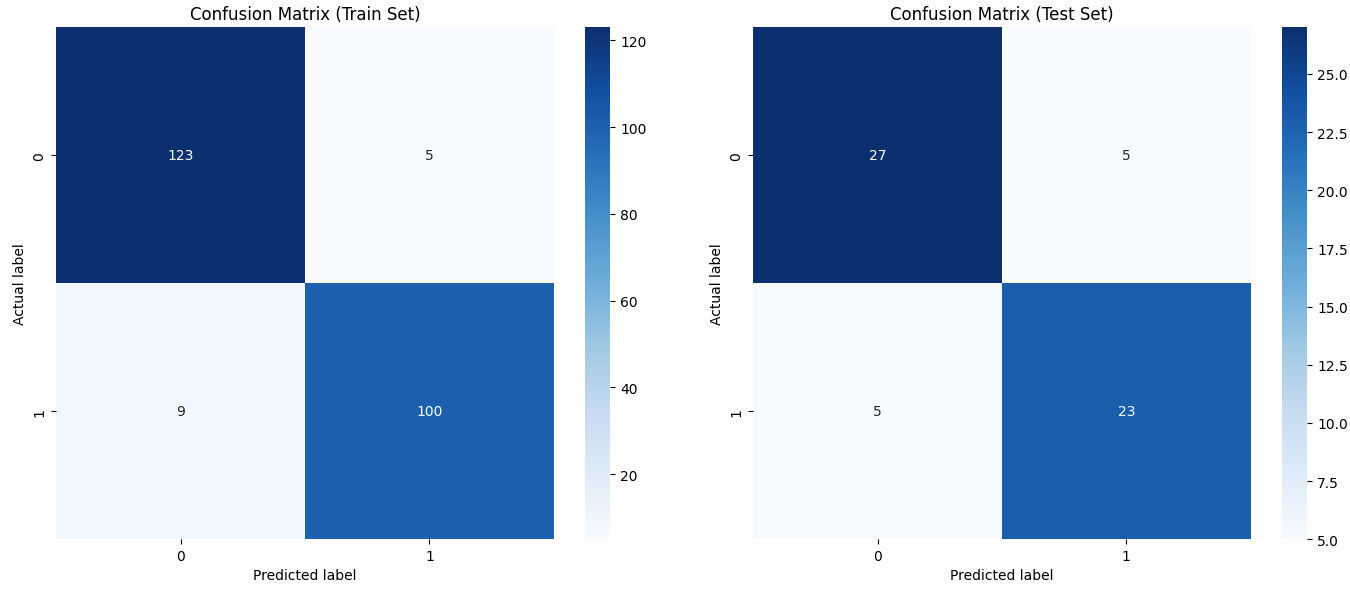
\includegraphics[width=1\linewidth]{images/confusion_matrix_mlp_base.png}
    \caption{Confusion Matrix}
    \label{fig:enter-label}
\end{figure}
\begin{figure}[H]
    \centering
    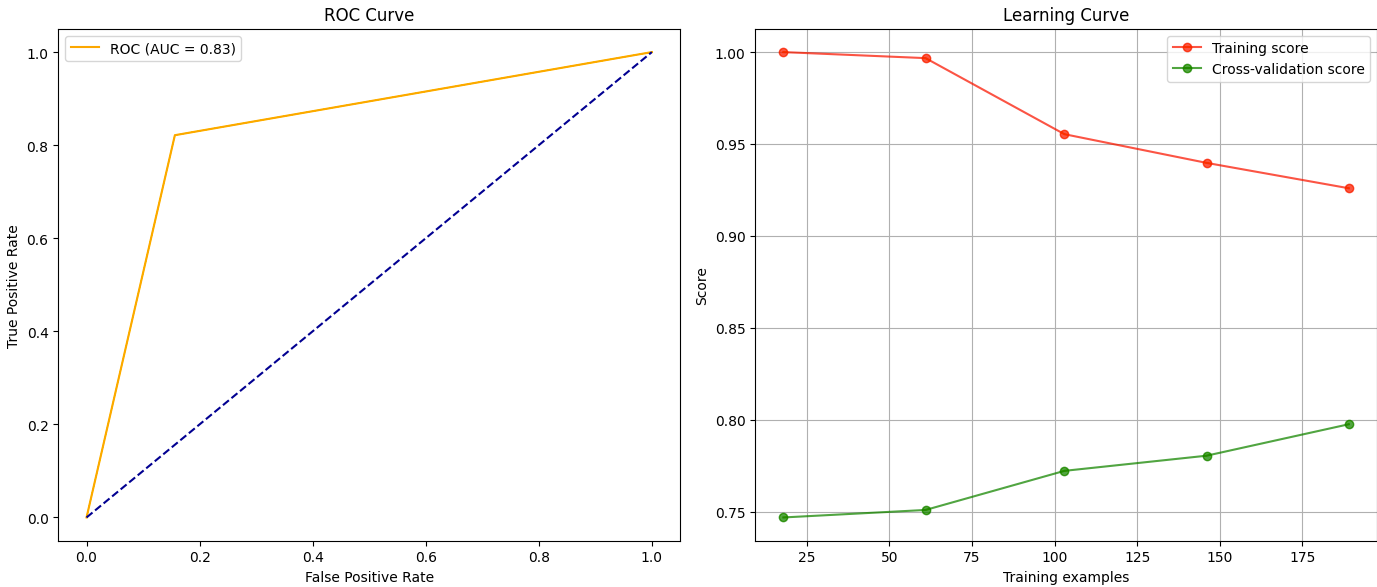
\includegraphics[width=1\linewidth]{images/roc_learning_mlp_base.png}
    \caption{ROC Curve and Learning Curve}%
    \label{fig:enter-label}
\end{figure}

\subsubsection{Hyper-Parameter Selection Model}

Next, we performed a search for the optimal values of the learning rate, alpha, and hidden layer sizes. These parameters play a critical role in determining the performance of the Multilayer Perceptron (MLP) model.

\begin{itemize} 
    \item \textbf{learning\_rate\_init}: Controls the initial step size for the gradient descent optimization process. Smaller values result in a slower, more stable convergence, while larger values speed up convergence but may cause instability or overshooting. 
    \item \textbf{alpha}: The regularization parameter, which controls the strength of L2 regularization. Higher values increase regularization and prevent overfitting, while smaller values allow the model to fit the training data more closely, potentially leading to overfitting. 
    
    \item \textbf{hidden\_layer\_sizes}: Specifies the number and size of hidden layers in the neural network. Larger networks with more neurons can capture more complex patterns but may also lead to overfitting. 
\end{itemize}

To find the optimal values for these parameters, we employed RandomizedSearchCV with the following ranges:

\begin{equation} learning\_rate\_init \in {0.001, 0.005, 0.01, 0.02} \end{equation} \begin{equation} alpha \in {0.0001, 0.001, 0.01} \end{equation} 
\begin{equation} hidden\_layer\_sizes \in {(10), (25), (50), (100), (10, 10), (20, 20)} \end{equation}

By using RandomizedSearchCV, we were able to efficiently explore the possible combinations of these hyperparameters and identify the best configuration for maximizing the model's performance.

\begin{table}[ht]
    \centering
    \caption{Best parameters in MLP} 
    \begin{tabular}{||c c c c||} 
     \hline
     alpha & hidden\_layer\_sizes & learning\_rate & max\_iter  \\ [0.5ex] 
     \hline\hline
     0.001 & (25,) & 0.001 & 200 \\ 
    \hline
    \end{tabular}
    \label{tab:tab2_mlp}
\end{table}

The results for the Hyper-Parameter Selection Model are:
\begin{figure}[H]
    \centering
    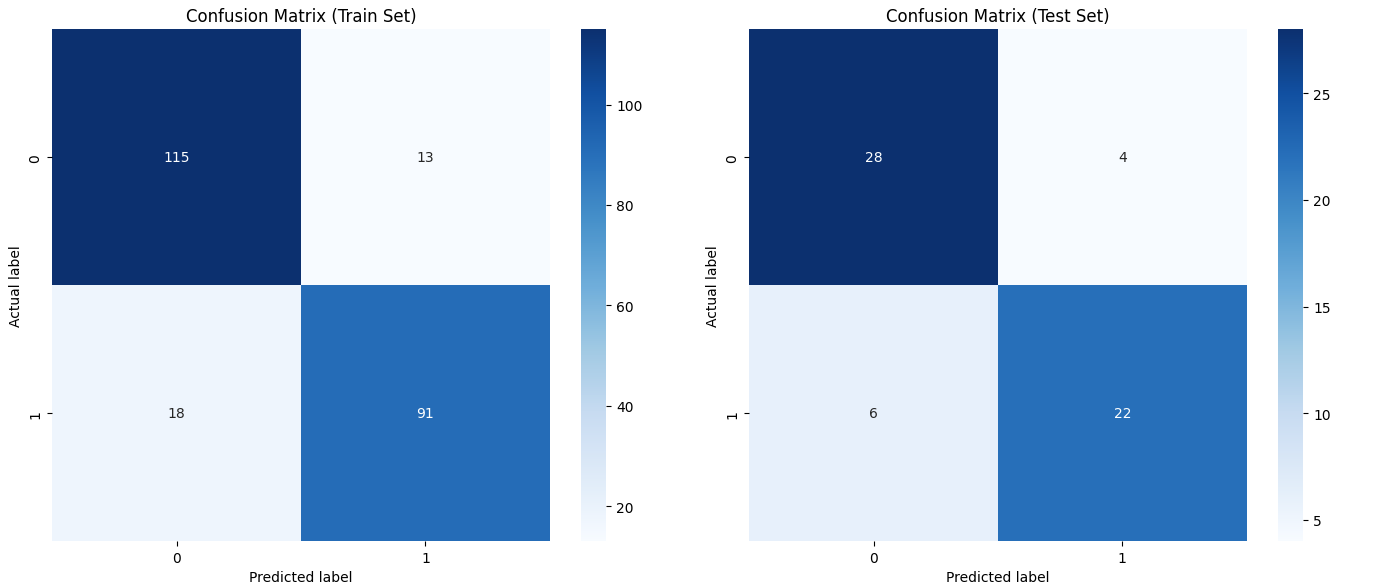
\includegraphics[width=1\linewidth]{images/confusion_matrix_mlp_search.png}
    \caption{Confusion Matrix}
    \label{fig:enter-label}
\end{figure}
\begin{figure}[H]
    \centering
    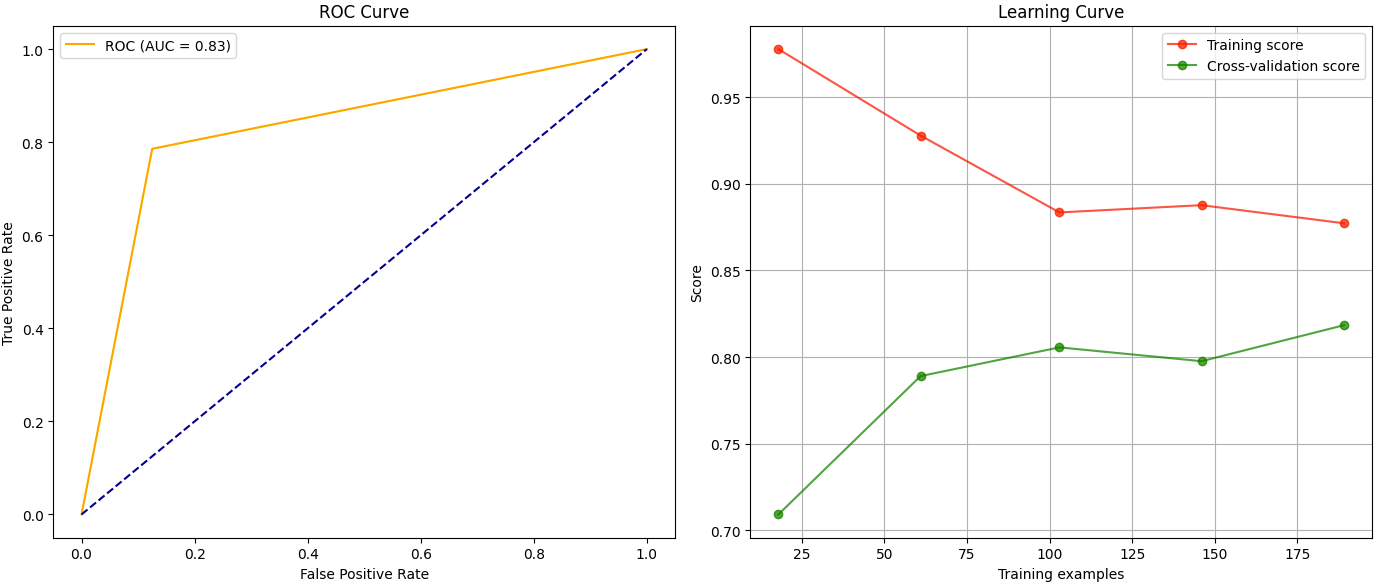
\includegraphics[width=1\linewidth]{images/roc_learning_mlp_search.png}
    \caption{ROC Curve and Learning Curve}%
    \label{fig:enter-label}
\end{figure}


\subsubsection{K-Fold Cross-Validation Model}

To evaluate the model's robustness and minimize the risk of overfitting, we applied K-Fold Cross-Validation. 

The results of the K-Fold Cross-Validation are shown in Figure \ref{fig:k_fold_cross_mlp.png}. Each fold's accuracy score is visualized, allowing us to identify the fold with the highest accuracy. In this case, the fold with the best performance was Fold 8, which achieved the highest accuracy.

\begin{figure}[H] \centering 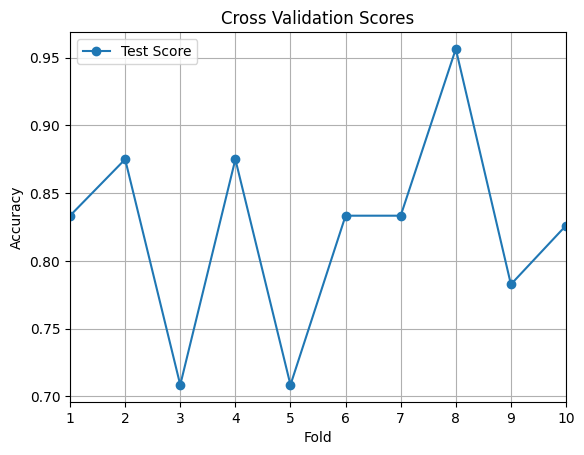
\includegraphics[width=0.75\linewidth]{images/k_fold_cross_mlp.png} \caption{Accuracy Scores Across K-Folds} \label{fig:k_fold_cross_svc.png} \end{figure}

Based on this result, the model corresponding to the best-performing fold (Fold 8) was selected and retrained on the entire training dataset. This ensures that the final model leverages all available training data while incorporating the insights gained from the cross-validation process.

The results for the K-Fold Cross-Validation Model are:

\begin{figure}[H]
    \centering
    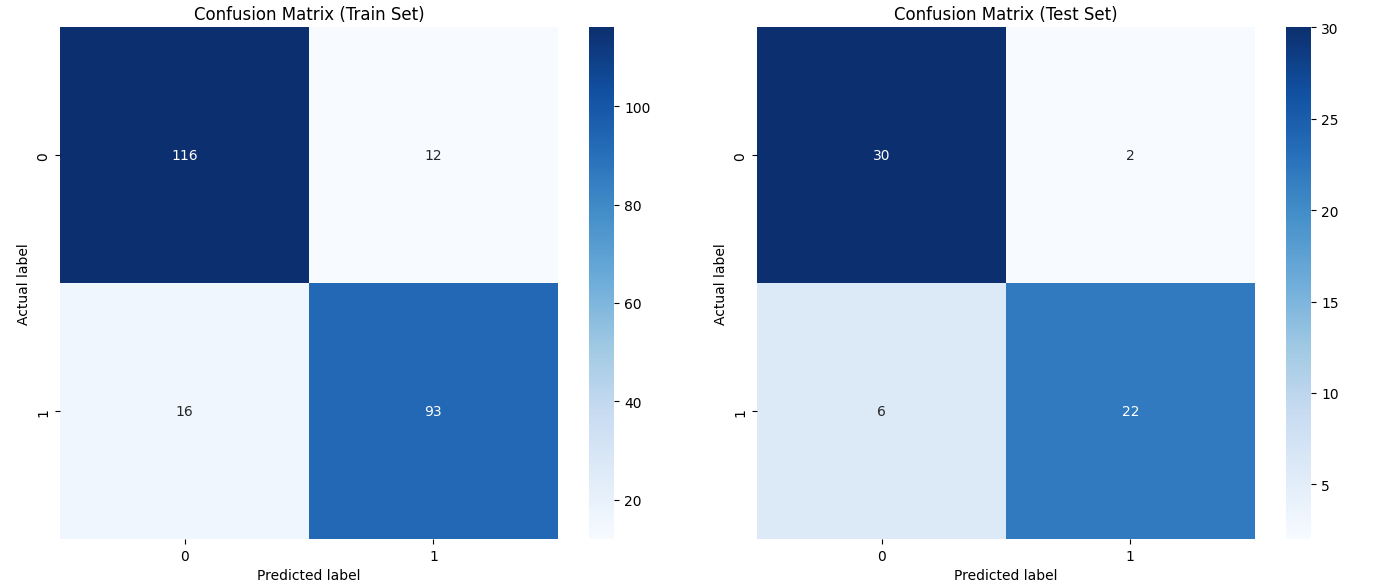
\includegraphics[width=1\linewidth]{images/confusion_matrix_mlp_kfold.png}
    \caption{Confusion Matrix}
    \label{fig:enter-label}
\end{figure}
\begin{figure}[H]
    \centering
    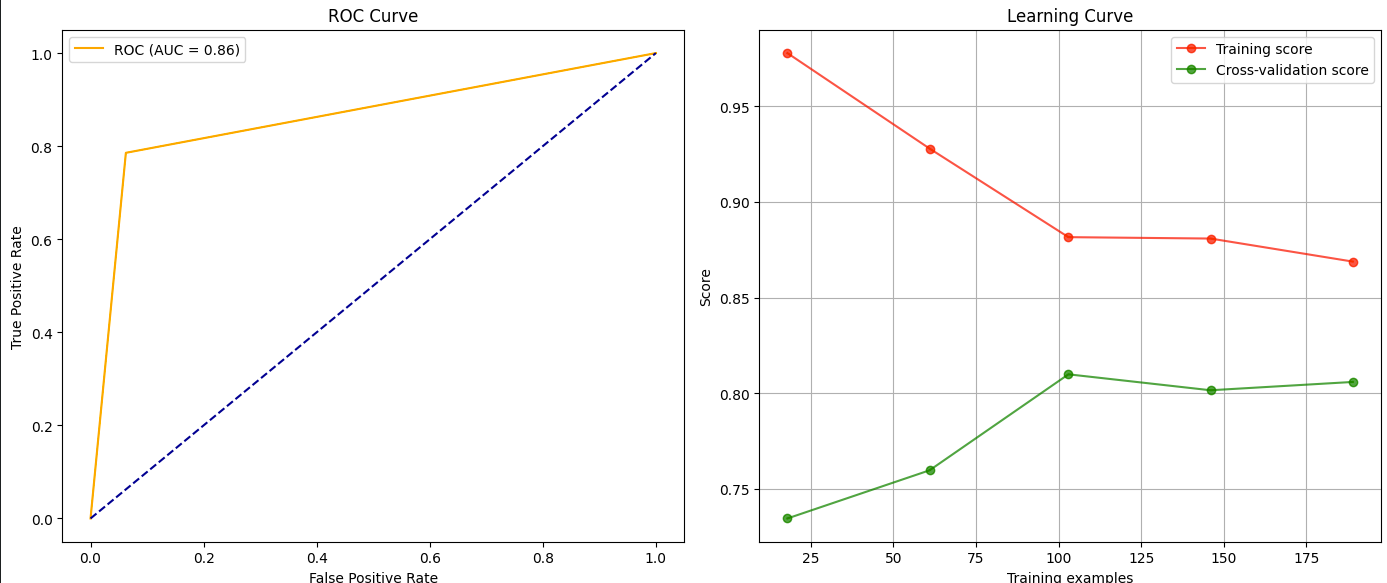
\includegraphics[width=1\linewidth]{images/roc_learning_mlp_kfold.png}
    \caption{ROC Curve and Learning Curve}%
    \label{fig:enter-label}
\end{figure}

\begin{figure}[H]
    \centering
    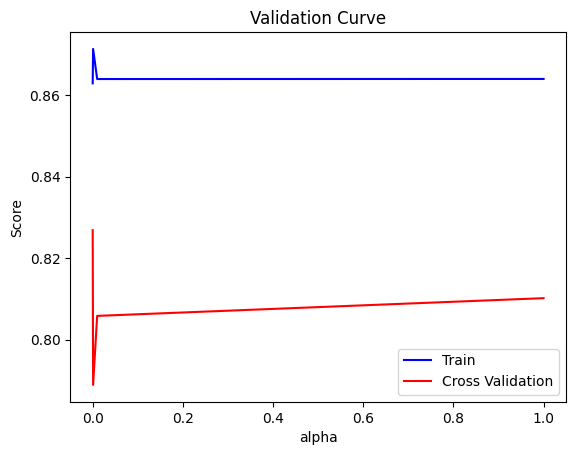
\includegraphics[width=0.75\linewidth]{images/ValidationCurveMLP_alpha.png}
    \caption{Validation Curve}
    \label{fig:ValidationCurveMLP_alpha}
\end{figure}
\begin{figure}[H]
    \centering
    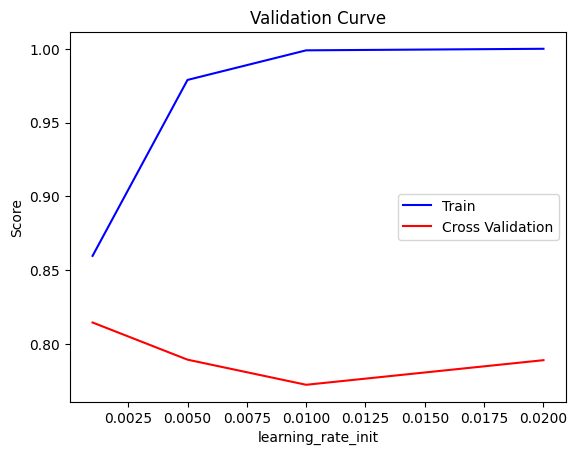
\includegraphics[width=0.75\linewidth]{images/ValidationCurveMLP_learning.png}
    \caption{Validation Curve}
    \label{fig:ValidationCurveGamma_SVC}
\end{figure}

\subsubsection{Conclusions}
As observed previously in the results, the confusion matrices show that the number of incorrectly classified examples, the sum of FP and FN, is very low compared to the number of correctly classified examples, the sum of TP and TN. This reinforces the model's accuracy and predictive power.

In addition, the AUC values for the MLP are slightly lower than those of other models, ranging between 0.83 and 0.86, but still indicating consistent and strong predictive power across both classifiers.

In Fig. \ref{fig:ValidationCurveMLP_alpha Curve}, we observe that alpha values in the range between 0 and 1 are suitable, with the best performance concentrated in the interval from 0 to 0.1. After a value close to 0, both training accuracy and cross-validation accuracy stabilize, with training scores around 0.86 and cross-validation scores around 0.80. This suggests that alpha values within this range provide a good balance between regularization and model fitting, ensuring that the model is neither too simple (underfitting) nor too complex (overfitting).

In the second graph, the analysis of the learning rate (learning\_rate\_init) shows that values between 0.0025 and 0.01 offer a good balance between training accuracy and cross-validation accuracy. Training scores reach up to 1.00, while cross-validation scores stabilize around 0.85, indicating that the model has learned well from the data without overfitting.

\begin{table}[H]
    \centering
    \caption{Classification - All Model} 
    \begin{tabular}{||c| c c c c||} 
     \hline
     & Accuracy & F1 Score & Recall & Precision \\
     \hline\hline
     Base Model & 0.833 & 0.821 & 0.821 & 0.821 \\
     \hline
    Hyper-Parameter & 0.833 & 0.815 & 0.786 & 0.846 \\ 
    \hline
    K-Fold & 0.868 & 0.846 & 0.786 & 0.917 \\ 
    \hline
    \end{tabular}
    \label{tab:tab_MLPFinal}
\end{table}

By examining Table \ref{tab:tab_MLPFinal}, we observe that the Accuracy and F1 Score for the Hyper-Parameter Selection Model and K-Fold Cross-Validation Model are identical, both slightly outperforming the Base Model. While the Base Model achieves a good Precision of 0.821, the Hyper-Parameter and K-Fold models improve this to 0.846 and 0.917, respectively. This indicates that the K-Fold model is the most effective at correctly identifying true positive cases among all positive predictions.

However, the Recall (or True Positive Rate) is slightly lower for the Hyper-Parameter and K-Fold models (0.786) compared to the Base Model (0.821), meaning the Base Model is marginally better at identifying actual positive cases, but at the cost of lower Precision.

The K-Fold model is the most preferable one because it has the highest values in all performance metrics except for recall where the differences are minimal in comparison with the other models.

\bigskip
\subsection{Comparison between the models}
The comparison between the models is based on the following performance metrics: Accuracy, F1 Score, Recall, and Precision. These metrics allow us to assess how well the models perform in terms of both correctly classifying positive and negative cases and minimizing false positives and false negatives.
\begin{itemize}
    \item \textbf{Accuracy} measures the overall correctness of the model by calculating the ratio of correct predictions to the total number of predictions.
    \item \textbf{F1 Score} is the harmonic mean of Precision and Recall, providing a balance between the two, especially when dealing with imbalanced classes.
    \item \textbf{Recall} (or True Positive Rate) measures the ability of the model to correctly identify positive instances.
    \item \textbf{Precision} measures the accuracy of positive predictions made by the model.
\end{itemize}

All models presented here underwent hyperparameter tuning using RandomizedSearchCV to find the optimal settings for each model. Additionally, K-Fold Cross-Validation was applied to ensure the robustness and generalizability of the results, providing a reliable estimate of how the models would perform on unseen data.

Below is the comparison table of the three models:

\begin{table}[H]
    \centering
    \caption{Comparison - All Model} 
    \begin{tabular}{||c| c c c c||} 
     \hline
     & Accuracy & F1 Score & Recall & Precision \\
     \hline\hline
     LR & 0.883 & 0.863 & 0.786 & 0.957 \\ 
     \hline
    SVC & 0.900 & 0.885 & 0.821 & 0.958  \\
    \hline
    MLP & 0.868 & 0.846 & 0.786 & 0.917 \\ 
    \hline
    \end{tabular}
    \label{tab:tab_Final}
\end{table}

Based on the results in Table \ref{tab:tab_Final}, we can observe the following:

\begin{itemize}
     \item The Logistic Regression (LR) model has an Accuracy of 0.883, an F1 Score of 0.863, and a Precision of 0.957. These results indicate that LR is effective at identifying true positive cases while maintaining a low rate of false positives.
    \item The Support Vector Classifier (SVC) model shows a higher Accuracy (0.900) and F1 Score (0.885) compared to the LR model, with Precision still being high (0.958). This suggests that SVC outperforms LR in terms of overall accuracy and balance between Precision and Recall.
    
    \item The MLP (Multilayer Perceptron), while having a lower Accuracy (0.868) and F1 Score (0.8463), still demonstrates good Precision (0.917). However, its overall performance is not as strong as SVC or LR.

\end{itemize}

The slightly lower performance of the MLP model can be attributed to several factors. One key reason could be the limited amount of training data available, which may not be sufficient to fully leverage the complexity of neural networks like MLP. Neural networks generally require large datasets to train effectively and avoid overfitting. Without enough data, the MLP model may not generalize well, which could explain its slightly lower performance compared to the SVC and LR models.

In this context, the SVC model emerges as the best performer, with the highest Accuracy and F1 Score, closely followed by LR. Both models show excellent Precision, making them suitable for applications where false positives must be minimized.
\section{Novelty and Contributions}
We found a published article by Ogunpola et al. (2024), \textit{Machine Learning-Based Predictive Models for Detection of Cardiovascular Diseases} \cite{ogunpola2024machine}, which investigates machine learning models for cardiovascular disease detection using the Cleveland Heart Disease Dataset and the MIMIC-III database. The authors emphasize the challenge of data imbalance in healthcare datasets and apply techniques such as resampling and cost-sensitive learning to address it.

This project focuses solely on the Cleveland Heart Disease Dataset, and we will compare our results with those obtained in the article. Their study evaluates several classifiers, including K-Nearest Neighbors, Support Vector Machines (SVM), Logistic Regression (LR), Convolutional Neural Networks (CNN), Gradient Boost, XGBoost, and Random Forest. In contrast, we have focused on evaluating only Logistic Regression (LR), Support Vector Machines (SVM), and Multi-Layer Perceptron (MLP).

We will compare performance metrics such as accuracy, precision, recall, and F1 score from our models with those reported in the literature.

\begin{table}[H]
    \centering
    \caption{Our Results} 
    \begin{tabular}{||c| c c c c||} 
     \hline
     & Accuracy & F1 Score & Recall & Precision \\
     \hline\hline
     LR & 0.883 & 0.863 & 0.786 & 0.957 \\ 
     \hline
    SVC & 0.900 & 0.885 & 0.821 & 0.958  \\
    \hline
    \hline
    \end{tabular}
    \label{tab:tab_our results}
\end{table}

\begin{table}[H]
    \centering
    \caption{Results from Article} 
    \begin{tabular}{||c| c c c c||} 
     \hline
     & Accuracy & F1 Score & Recall & Precision \\
     \hline\hline
     LR & 0.885 & 0.885 & 0.844 & 0.931 \\ 
     \hline
    SVC & 0.787 & 0.794 & 0.781 & 0.807 \\
    \hline
    \hline
    \end{tabular}
    \label{tab:tab_our results}
\end{table}

By analyzing the performance metrics (accuracy, F1 score, recall, and precision) from our models and the results in the article, we can make the following observations:
\\
The performance of \textbf{Logistic Regression (LR)} in our model is very similar to the one reported in the article, with a marginal difference in accuracy (our result is slightly lower by 0.002). Our precision (0.957) is slightly better, but their recall (0.844) and F1 score (0.885) are higher, indicating that their model was able to identify more truly positive cases and had a better overall balance between precision and recall.

Our \textbf{SVC} model significantly outperforms the \textbf{SVC} model from the article in all metrics. Our model shows a much higher accuracy (0.900) and precision (0.958), suggesting that the SVC model in our project is more effective at identifying true positives while maintaining a low rate of false positives. Additionally, our recall (0.821) is higher than the article's model (0.781), which indicates that our model performs slightly better in identifying actual positive cases.

 Our models show strong performance, but the differences in the results indicate areas for potential improvement, especially in handling data imbalance and optimizing recall. Techniques such as resampling and cost-sensitive learning, as used in the article and could be useful to enhance performance, where recall can be further improved. Additionally, feature selection and further hyperparameter tuning may also help in refining the models for better overall performance.
\input{3-conclusão}
% printing acronyms
%\printglossary[type=\acronymtype,title=Acronyms]

% references section
\bibliography{refs}
\bibliographystyle{IEEEtran}



\end{document}